% ============================================================================
% ONR FY2027 Young Investigator Program (YIP), Technical Proposal (Volume 1)
% ALTERNATIVE VERSION: seawater-resistant copper alloys designed as powders for
% single-stream, blown-powder directed energy deposition (DED).
% NOFO N0001426SF004 (posted 17 Aug 2026, file FY27_YIP_NOFO_N0001426SF004__003.pdf)
% Due 30 Oct 2026, 5:00 PM Eastern, via Grants.gov (NOFO p. 27).
%
% This file is an alternative to onr-yip-technical-proposal.tex (aluminum
% alloys, laser powder bed fusion). Only one of the two would be submitted.
% Kept from the aluminum version: the linked-model, cost-aware search
% (Advances 1, 2 and 5 here; H1, H2 and H4), the staged specimens with a 99%
% density gate, the audit of screened-out candidates, the synthetic benchmark
% (Figs. 2 and 3, still aluminum), and the management, responsibility, and
% data sections. Changed: the alloy system and naval application (70-30
% copper-nickel and nickel-aluminum bronze replacements), the process (DED,
% with a repair branch), the powder step (sized and checked for blown
% powder), the physics inputs (CALPHAD along the DED thermal history, new
% Advance 3 and H3), and the corrosion tests (seawater screen, then
% immersion). See README.md, "Alternative: copper alloys for blown-powder DED".
%
% Format, page limit, required sections, and page numbering are as in
% onr-yip-technical-proposal.tex (NOFO pp. 15-20): 8.5 x 11 in, 1 in margins,
% single-spaced, Times New Roman 12 pt, 20 counted pages.
%
% The cover gives the copper budget from SPO's planning sheet of 23 Oct 2026,
% with a TODO for the final figures; the budget macros
% (budget/budget-numbers.tex) are the aluminum version's and are no longer
% used here. Facility rates for the Utah and Mines DED sessions stay in the
% private budget, not in this repository.
%
% Red [TODO Sterling: ...] markers are guesses or facts not yet confirmed.
%
% Build: xelatex onr-yip-technical-proposal-cu-ded.tex (twice)
% ============================================================================

\documentclass[12pt,letterpaper]{article}

\usepackage[margin=1in]{geometry}
\usepackage{iftex}
\ifPDFTeX
  \usepackage[T1]{fontenc}
  \usepackage[utf8]{inputenc}
  \usepackage{mathptmx}
\else
  \usepackage{fontspec}
  \IfFontExistsTF{Times New Roman}
    {\setmainfont{Times New Roman}}
    {\setmainfont{TeX Gyre Termes}}
\fi
\usepackage{microtype}
% Let TeX stretch spaces instead of pushing lines into the 1-inch margin.
\setlength{\emergencystretch}{3em}

\setlength{\parindent}{0pt}
\setlength{\parskip}{5pt plus 2pt minus 1pt}
\setlength{\textfloatsep}{10pt plus 2pt minus 2pt}

\usepackage{graphicx}
\usepackage{xcolor}
\usepackage{tikz}
\usetikzlibrary{positioning,arrows.meta,fit}
\usepackage{array}
\usepackage{booktabs}
\usepackage{tabularx}
\usepackage{pdfpages}
\usepackage[labelfont=bf,labelsep=period,skip=4pt]{caption}
\usepackage{xurl}
\usepackage[colorlinks=true,linkcolor=blue!70!black,citecolor=blue!70!black,
  urlcolor=blue!70!black]{hyperref}

\usepackage{titlesec}
\titleformat{\section}{\normalfont\normalsize\bfseries}{\thesection.}{0.5em}{}
\titlespacing*{\section}{0pt}{10pt plus 2pt minus 2pt}{2pt}
\titleformat{\subsection}{\normalfont\normalsize\bfseries}{\thesubsection}{0.5em}{}
\titlespacing*{\subsection}{0pt}{8pt plus 2pt minus 2pt}{1pt}
\titleformat{\subsubsection}[runin]{\normalfont\normalsize\bfseries}{}{0pt}{}[.]
\titlespacing*{\subsubsection}{0pt}{5pt plus 2pt minus 1pt}{0.5em}

\pagestyle{plain}
\newcommand{\todo}[1]{\textcolor{red}{[TODO Sterling: #1]}}
\hyphenation{re-POW-DER AMA-ZE-MET}

\newcommand{\BudgetTotal}{747,651}
\newcommand{\BudgetYearOne}{248,959}
\newcommand{\MTDCYearOne}{140,298}
\newcommand{\FAYearOne}{72,253}
\newcommand{\BuildsYearOne}{28}
\newcommand{\BudgetYearTwo}{248,828}
\newcommand{\MTDCYearTwo}{151,728}
\newcommand{\FAYearTwo}{78,140}
\newcommand{\BuildsYearTwo}{29}
\newcommand{\BudgetYearThree}{249,864}
\newcommand{\MTDCYearThree}{152,036}
\newcommand{\FAYearThree}{78,299}
\newcommand{\BuildsYearThree}{26}

\begin{document}

% ===========================================================================
% Cover page (excluded from the page limit)
% ===========================================================================
\pagenumbering{roman}
\begin{titlepage}
\begin{center}
{\Large\bfseries Technical Proposal\par}
\vspace{10pt}
{\large\bfseries Cost-Aware Design of Seawater-Resistant Copper Alloy\\
Powders for Blown-Powder Directed Energy Deposition\par}
\vspace{10pt}
Office of Naval Research (ONR)\\
Fiscal Year 2027 Young Investigator Program (YIP)
\end{center}
\vspace{12pt}
\renewcommand{\arraystretch}{1.25}
\begin{tabular}{@{}>{\bfseries\raggedright\arraybackslash}p{1.95in}>{\raggedright\arraybackslash}p{4.3in}@{}}
NOFO number & N0001426SF004 \\
Title & Cost-Aware Design of Seawater-Resistant Copper Alloy Powders for
  Blown-Powder Directed Energy Deposition \\
Prime applicant & Brigham Young University (BYU), Provo, Utah \\
Subawardees & None \\
ONR S\&T Focus Areas & Primary: Manufacturing (Integrated Manufacturing and
  Sustainment Technologies). Secondary: Materials and Electronics
  (Sustainable and Operationally Robust Materials). \\
ONR program & Materials \& Processes for Additive Manufacturing, Code 332
  (Dr.~Charles Fisher) \\
Technical contact & Sterling G.\ Baird, Ph.D., Assistant Professor,
  Department of Mechanical Engineering, Brigham Young University, 350 EB,
  Provo, UT 84602. Phone (801) 422-5344. Email
  \href{mailto:sterling.baird@byu.edu}{sterling.baird@byu.edu} \\
Administrative and business contact & \todo{name, title, address, phone,
  and email of the BYU Research Administration officer who signs as the
  Authorized Organization Representative} \\
Period of performance & Base period only, 36 months: 1 April 2027 to
  31 March 2030. No option periods. \\
Requested amount & \$748,087 total: \$248,883, \$249,638, and \$249,566
  in the three 12-month periods \todo{the copper budget on SPO's planning
  sheet of 23 Oct 2026; final figures from BYU
  Research Administration} \\
\end{tabular}
\end{titlepage}

% ===========================================================================
% Table of contents (excluded from the page limit)
% ===========================================================================
\setcounter{page}{2}
\setcounter{tocdepth}{2}
\tableofcontents
\clearpage

% ===========================================================================
% Pages 1 to N count toward the 20-page limit
% ===========================================================================
\pagenumbering{arabic}

\section{Technical Approach}

% Epigraph: verbatim from the NAVSUP WSS article of 30 Jun 2026 (navsup2026),
% which quotes the CNO's remarks to the Surface Navy Association earlier in 2026.
\begin{flushright}
\begin{minipage}{4.9in}
\itshape ``Over the last year, we placed nearly 120 additive manufacturing
parts into development, installed 20 of those parts, and eliminated more than
1,400 cumulative days of delay.''\par
\vspace{2pt}\upshape\hfill Adm.\ Daryl Caudle, Chief of Naval Operations,
2026~\cite{navsup2026}
\end{minipage}
\end{flushright}

\subsection{Problem and objectives}

In the Navy, much of the seawater service runs on two kinds of copper alloy.
Copper-nickel alloys, 90-10 (UNS C70600) and 70-30 (UNS C71500), carry
seawater in piping, condensers, and heat exchangers, and nickel-aluminum
bronze (NAB, UNS C95800) is cast into propellers, valves, and pump
parts~\cite{milt16420,milb24480,cda222}. Both were developed for casting or wrought processing.
Directed energy deposition (DED), in which a laser melts a stream of powder
blown into a moving melt pool, can build large parts and restore worn or
damaged ones without a foundry~\cite{saboori2019,cao2019}. DED, however, cools each
layer from the melt within seconds and reheats it many times as later layers
pass, so it produces microstructures these alloys were never designed for. In
NAB, fast cooling can retain a martensitic phase that corrodes selectively in
seawater~\cite{liu2021,dobson2024}, and the Navy specification for NAB deposited
by wire-arc DED requires the same 6-hour anneal as castings~\cite{milprf32816}.
That step is costly for a large part and impractical for many repairs made in
place. Navy specifications for printed copper alloys all use existing
compositions~\cite{milprf32816,milprf32804,milprf32815}, and the design of
compositions for laser deposition has only begun~\cite{jia2026}.

Designing one runs through a chain of steps: a thermodynamic calculation, a
powder, deposited test specimens, microscopy, and property tests. The costs of
the steps differ greatly. A thermodynamic calculation takes minutes, a powder
lot a day, a DED session days including turnaround, and a corrosion immersion
weeks. The protective film that gives copper-nickel its resistance takes weeks
to months to mature~\cite{ma2015,ekerenam2018}. Experimental campaigns often send each
candidate through the whole chain, spending much of the budget on full tests
of candidates that a cheap early measurement could have ruled out.
Computational campaigns often work as a funnel: many simulations, then a few
candidates passed on to experiments. If the simulation misses a physical
effect, the funnel discards good candidates before any experiment can catch
the error.

The powder is a second obstacle. Single-stream blown-powder DED, the form in
use today, feeds a pre-alloyed powder from one hopper. Each new composition
therefore needs its own powder lot, in a size range that flows through the
nozzle and that the melt pool catches~\cite{ancalmo2025,singh2020}. The lot must also
fill the hopper, about 2~kg on the larger of the two systems this project
will use (Section~\ref{sec:task2}).
Industrial gas atomizers make powder in lots of tens of kilograms or more, so
new compositions are rarely tried \todo{cite a minimum lot size, e.g., a
vendor's}. Our ultrasonic atomizer makes a lot of a new composition in a day
from about half a kilogram of feedstock, and 2~kg in about six runs. Ultrasonic
atomizers have already made powder for blown-powder DED from NAB
propeller grinding chips~\cite{muller2023,uhlmann2024} and from copper cable
scrap~\cite{cabrioli2025}, but only in existing compositions. That turns
the powder from a purchase into steps the search can choose. A small lot is
enough for cheap deposits of many compositions on a small DED system near BYU.
A full lot is made only for those worth building on the larger system. It
also lets the search design the powder along with the alloy.

This project asks a basic question. When the steps of a materials workflow
differ in cost by orders of magnitude, and results arrive at different times,
how should one choose the next measurement and the next candidate? It also
asks a materials question. How do composition and the DED thermal history
together set segregation, cracking, fusion to a substrate, and corrosion in
an as-deposited copper alloy? We answer both on a concrete design problem: a
pre-alloyed copper alloy powder for single-stream blown-powder DED. The
powder must deposit without cracks or pores, on itself and on the alloys it
would repair, and the deposit must resist seawater without heat treatment at
least as well as 70-30 copper-nickel. Repair of cast NAB and wrought
copper-nickel is the demanding test of both answers.
The project has five objectives:
\begin{enumerate}\setlength{\itemsep}{0pt}
\item Extend a cost-aware search method that learns from partial results to
several competing objectives: dense and crack-free deposits, strength,
ductility, and resistance to corrosion in seawater.
\item Extend it to many experiments in progress at once, with results that
return at different times.
\item Give it physics computed for the process, thermodynamic calculations
evaluated along the thermal history of a DED deposit, and measure what that
physics is worth.
\item Demonstrate the method on a physical workflow that designs copper alloy
powders for blown-powder DED, from powder to deposit, repair coupon, tensile
test, and seawater corrosion test. Test whether its stated confidence in a
candidate matches what the deposits and tests later show.
\item Measure how well a one-hour electrochemical screen predicts immersion
tests that take weeks, so that the long tests run only where they can change
a decision.
\end{enumerate}

\subsection{Copper alloys in naval seawater service}
\label{sec:naval-cu}

Navy specifications cover copper-nickel tube for the piping systems of
surface ships and submarines~\cite{milt16420} and NAB castings for seawater
service~\cite{milb24480}. NAB is widely used for valve bodies, pump
casings, and impellers, with a large market in submarine
fleets~\cite{cda222}. Copper-nickel owes its resistance to a thin, adherent
film of corrosion products, mainly cuprous oxide with nickel and iron. The
film builds up over weeks to months of exposure~\cite{ma2015}. In one study the
films on 90-10 tubes in natural seawater were still changing after six
months~\cite{ekerenam2018}. The iron content of the alloy changes the makeup
of the film~\cite{zhu2021}. NAB is a cast alloy of copper with about 9\%
aluminum and 4 to 5\% each of iron and nickel (by weight). Its microstructure
of $\alpha$ grains and several intermetallic $\kappa$ phases resists seawater
well, but the $\alpha$ phase in the lamellar $\alpha+\kappa$ eutectoid, and
any retained $\beta$ phase, corrode selectively, above all in
crevices~\cite{wharton2005,culpan1979}. Navy NAB castings therefore get a temper
anneal at 1250 $\pm$ 50\,\textdegree{}F (about 677\,\textdegree{}C) for at
least 6 hours, propellers excepted~\cite{milb24480}, which improves their
corrosion resistance~\cite{cda222}.

Printing changes these microstructures, and printing changes how alloys
corrode~\cite{sander2018}. How NAB is processed sets its
microstructure~\cite{orzolek2022}, and NAB has now been printed by laser
powder bed fusion~\cite{murray2020}, wire-arc deposition~\cite{ding2016,dharmendra2019},
and laser DED~\cite{liu2021,li2021}. Laser-deposited NAB contains martensitic
$\beta'$ along with $\alpha$ and $\kappa$ phases~\cite{liu2021,li2021} and
is much stronger than cast NAB~\cite{li2021}. Its corrosion depends on the
process. NAB from laser powder bed fusion formed stronger films than wrought
NAB but resisted localized corrosion worse, and annealing reversed
both~\cite{morshed2024}. Wire-arc NAB corroded in its residual $\beta$
phase~\cite{cai2023}. Whether annealing helps depends on the starting
microstructure. After 480 hours in salt solution, the same 700\,\textdegree{}C
anneal had lowered the corrosion current of cast NAB and raised that of
sintered and hot isostatically pressed NAB, each about
threefold~\cite{fayanas2025}. The authors call the differences small. As-built wire-arc NAB
resisted corrosion better than annealed coupons, in a test with unequal
immersion times~\cite{shahriari2023}. Laser-deposited NAB on stainless steel
was attacked to a depth of 3.4\,$\mu$m in 21 days in salt solution where iron
from the steel had diluted it, and 1.8\,$\mu$m over a nickel-chromium
interlayer~\cite{zhao2022}. In welded NAB,
retained $\beta'$ in the heat-affected zone corroded selectively in
seawater~\cite{dobson2024}, a warning for repairs. Laser cladding of cast
NAB has used an NAB consumable~\cite{hyatt1998}, and DED repair of cast NAB
a low-nickel copper alloy powder~\cite{yao2022a,yao2022b}. That powder was
later blended in the melt pool with an aluminum alloy powder to vary the
aluminum content~\cite{yao2025}.

In wire-arc 70-30 copper-nickel, the dendrite cores hold more nickel than the
regions between them, and those regions corrode first~\cite{song2024}. The
corrosion of powder-bed 70-30 has also been studied~\cite{liu2024}, and its
resistance depends on the laser settings~\cite{nadimi2025}. At their best
settings, both wire-arc and powder-bed 70-30 have matched or beaten wrought
plate in electrochemical tests in salt solution~\cite{song2024,nadimi2025}.
Laser cladding of Cu-30Ni dates to 2005~\cite{adak2005}, and later
blown-powder DED of copper-nickel has mixed copper and nickel-alloy powders
in the melt pool to make graded layers and thermoelectric
alloys~\cite{karnati2019,yadav2020,williams2025}. The one corrosion study
we found of copper-nickel deposited by blown-powder laser DED is from 2011:
Cu-30Ni made by CO$_2$-laser direct metal deposition on wrought 70-30
plate~\cite{bhattacharya2011}. A later review reports that the deposit
corroded faster than the plate and attributes this to its
porosity~\cite{issc2012} \todo{check the 2011 article before citing a
direction. Read literally, its abstract ranks the deposit as the most
corrosion resistant and the plate as the least, the reverse of the review. A
secondary source found by web search quotes ASTM G31 rates of 0.36~mpy for
the deposit and 0.08~mpy for the plate. Neither Edison nor this runner could
open the article}. NAVSEA has written specifications for 70-30 copper-nickel made by
wire-arc DED and by laser powder bed fusion, and for NAB made by wire-arc DED.
The wire-arc ones are alternatives to castings, and all three keep the
existing compositions~\cite{milprf32816,milprf32804,milprf32815}. We found none for
either alloy made by blown-powder laser DED. In 2023 a Navy official said,
as Defense News reported, that for naval metals ``including copper-nickel,''
``more research is needed'' on how printing ``affects the metals' fatigue and
corrosion properties''~\cite{defensenews2023}. A composition chosen for casting is not
necessarily the best one for DED, and each composition and set of deposition
settings needs its own tests.

Corrosion tests of copper alloys follow the same cost pattern as the rest of
the workflow. Open-circuit potential, linear polarization, and impedance
measurements in substitute ocean water~\cite{astmD1141} take about an hour and
give a corrosion rate and a measure of the surface film~\cite{astmG59,astmG102}.
Immersion tests with mass loss~\cite{astmG31,astmG1} and cross-sections that
measure the depth of selective attack take weeks. Tests in flowing seawater,
which set the velocity limits used in piping design, take months. The search
can therefore treat corrosion the way it treats cracking and strength: a cheap
screen for many candidates and long tests for a few. The cheap screen can
mislead, though. An hour-long measurement on a fresh surface sees neither the
film that forms over weeks on copper-nickel nor slow selective attack in NAB.
On wrought 70-30 copper-nickel in synthetic seawater, the corrosion current
fell more than eightfold over the first ten days~\cite{yuan2007}, and welded
NAB corroded faster in natural seawater than in simulated
seawater~\cite{dobson2024b}. In a study with NSWC Carderock, Volta potentials
measured in air on NAB plate ranked its phases backwards: the phase with the
highest potential was the one attacked in solution~\cite{iannuzzi2017}.
Knowing when the screen can be trusted is part of the research.

Supply and melting add one more objective. Nickel has been on the U.S. list
of critical minerals since 2022, and copper joined it in
2025~\cite{usgs2022,usgs2025}. Nickel also raises the melting range: 70-30
copper-nickel melts between about 1,171 and 1,238\,\textdegree{}C, 90-10
between 1,099 and 1,149\,\textdegree{}C, and NAB between 1,043 and
1,060\,\textdegree{}C~\cite{cdadata}. A replacement for 70-30 copper-nickel
that needs less nickel would use less of a critical mineral and would be
easier to atomize and deposit. The search will carry nickel content as an
objective to minimize where the corrosion trade-offs allow.

\subsection{Scientific concepts}
\label{sec:concepts}

The search method treats the manufacturing workflow as a network of linked
models~\cite{astudillo2021}. Each step gets its own statistical model (a
Gaussian process), which predicts the outputs of that step and how uncertain
they are. The models are linked in the same order as the steps
(Fig.~\ref{fig:network}), so the outputs of one step are inputs to the next
and uncertainty carries through the whole network. Because each step has its
own model, the network learns from partial results, and a candidate can stop
at any step. Buathong et al.\ added a cost-aware rule to this
network~\cite{buathong2024}. For each possible experiment, the rule estimates
how much the result is expected to improve the search, divides that by the
cost of the experiment, and runs the best one. In this project the deposition
step is itself split in two by cost. A small DED system at the University of
Utah, 45 miles from BYU, deposits tracks, walls, and small blocks from grams
to half a kilogram of powder on a day trip. A larger one at the Colorado
School of Mines, 500 miles away, builds tensile, corrosion, and repair
specimens from 2~kg lots, with results in weeks. Our rule treats the two as
linked steps with their own costs and pays for the larger one only where the
smaller one shows that a composition could change the outcome
(Section~\ref{sec:task2}).

The physics comes first, in the manner of integrated computational materials
engineering (ICME)~\cite{olson1997,nrc2008}: calculations decide where
experiments go, and experiments correct the calculations. Calculation of
phase diagrams (CALPHAD) in Thermo-Calc and pycalphad~\cite{andersson2002,otis2017}
gives the liquidus and freezing range of each composition and an index of how
prone it is to cracking as it solidifies~\cite{kou2015}. Such indices have
been checked against printed aluminum alloys, steels, and nickel
superalloys, but not copper alloys~\cite{jordan2026}. It also gives how
nickel, iron, and aluminum divide between the dendrite cores and the last
liquid to freeze, and the phases stable at each temperature, including the $\beta$ and $\kappa$ phases of the
bronzes. DED adds a thermal history. For each set of deposition settings, a
moving point-source model of heat flow~\cite{rosenthal1946,pinkerton2015}
gives the cooling rate through solidification and the peak temperatures that
later passes impose on each layer. We calibrate it to measured melt-pool
sizes and give it the temperature-dependent properties that NSWC Carderock
has measured for 70-30 and 90-10 copper-nickel and for NAB plate and
wire-arc NAB~\cite{norkett2025,norkett2026a,orzolek2023,norkett2026b}.
Room-temperature constants in their place can reverse the predicted
distortion of a NAB deposit~\cite{hatala2021}. For new compositions, which
these databases do not cover, we estimate the properties from the nearest
measured alloy and CALPHAD and carry the added uncertainty into the model.
The CALPHAD
calculations are then evaluated at those temperatures, to estimate which
phases can form as the deposit solidifies and which can form or dissolve as
it is reheated. These outputs enter the statistical models as inputs with
learned weights, so the search can discount any of them that proves
uninformative. The calculations run continuously on BYU high-performance
computing, and each new result is available to the next decision.

\begin{figure}[t]
\centering
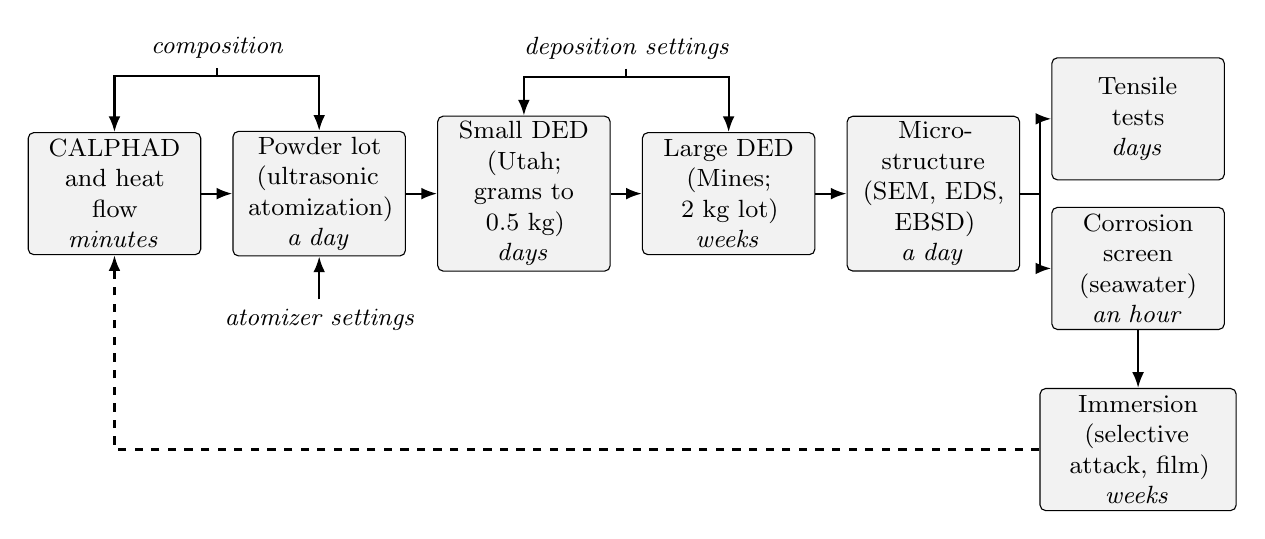
\begin{tikzpicture}[
  font=\small,
  box/.style={draw, rounded corners=2pt, fill=black!5, align=center,
    text width=2.05cm, minimum height=1.55cm, inner sep=2pt},
  arr/.style={-{Latex[length=2mm]}, thick},
  input/.style={font=\small\itshape, align=center}
]
\node[box] (s1) at (0,0) {CALPHAD\\and heat\\flow\\\textit{minutes}};
\node[box] (s2) at (2.6,0) {Powder lot\\(ultrasonic\\atomization)\\\textit{a day}};
\node[box] (s3) at (5.2,0) {Small DED\\(Utah;\\grams to\\0.5~kg)\\\textit{days}};
\node[box] (s4) at (7.8,0) {Large DED\\(Mines;\\2~kg lot)\\\textit{weeks}};
\node[box] (s5) at (10.4,0) {Micro-\\structure\\(SEM, EDS,\\EBSD)\\\textit{a day}};
\node[box] (s6) at (13.0,0.95) {Tensile\\tests\\\textit{days}};
\node[box] (s7) at (13.0,-0.95) {Corrosion\\screen\\(seawater)\\\textit{an hour}};
\node[box, text width=2.35cm] (s8) at (13.0,-3.25) {Immersion\\(selective\\attack, film)\\\textit{weeks}};
\foreach \a/\b in {s1/s2, s2/s3, s3/s4, s4/s5, s7/s8} \draw[arr] (\a) -- (\b);
\draw[arr] (s5.east) -- ++(0.25,0) |- (s6.west);
\draw[arr] (s5.east) -- ++(0.25,0) |- (s7.west);
\node[input] (comp) at (1.3,1.85) {composition};
\draw[arr] (comp.south) -- ++(0,-0.1) -| (s1.north);
\draw[arr] (comp.south) -- ++(0,-0.1) -| (s2.north);
\node[input] (atom) at (2.6,-1.6) {atomizer settings};
\draw[arr] (atom) -- (s2);
\node[input] (dep) at (6.5,1.85) {deposition settings};
\draw[arr] (dep.south) -- ++(0,-0.1) -| (s3.north);
\draw[arr] (dep.south) -- ++(0,-0.1) -| (s4.north);
\draw[arr, dashed] (s8.west) -| (s1.south);
\end{tikzpicture}
\caption{The workflow as linked models, with typical times per result in
italics. DED is bought at two facilities that the search treats as two steps
of different cost. The small system at Utah melts pre-placed tracks from
grams of a first powder lot, then blown-powder tracks, walls, and small
blocks from about 0.5~kg. A composition that earns it is scaled up to the
2~kg lot that the hoppers of the large system at Mines need, for tensile,
corrosion, and repair specimens. That takes weeks, including the extra
atomizer runs and turnaround at the facility.
Composition enters at the first two steps, atomizer settings at the second,
and deposition settings (laser power, travel speed, and for blown powder the
feed rate) at the third and fourth. The heat flow model also takes the
deposition settings. After microscopy the network branches to tensile tests
and to corrosion tests. Dashed arrow: each result updates the models, which
choose the next experiments and steps by expected gain per cost.}
\label{fig:network}
\end{figure}

\subsection{Comparison with other approaches}

To our knowledge, no cost-aware search over linked models that can stop a
candidate at any step has been extended to several objectives or to results
that arrive out of order. None has been demonstrated on a physical alloy
workflow.
Published tests of the linked-model methods use test functions and
simulators~\cite{astudillo2021,buathong2024}. Multi-stage Bayesian
optimization for self-driving laboratories was tested on synthetic and
past data with one objective~\cite{torresi2026}. Cost-aware batch
optimization of refractory alloys treats measurements of unequal cost as
separate sources rather than linked steps, in a computational
campaign~\cite{alvi2026}. Closed-loop campaigns on printed alloys use one
model and a fixed set of measurements~\cite{talbot2026}. A search guided by model
uncertainty has chosen compositions of multi-principal element alloys
deposited by DED, scored on hardness~\cite{nelaturu2024}. One model has
combined a cheap analytical heat-flow model with costlier finite-element
simulations to map DED settings~\cite{menon2022}. Neither linked the steps or their costs. Alloys designed for
printing by computation, such as an oxide-dispersion-strengthened NiCoCr
alloy~\cite{smith2023} and high-strength aluminum
alloys~\cite{thapliyal2020,taheri2025}, were designed and then printed as
single compositions. An ONR-funded CALPHAD-based ICME framework screened
450,000 compositions of a naval steel for the chance of a successful print
under the scatter of powder composition~\cite{wang2020}. It worked from
composition and heat treatment, without the thermal history of the build,
corrosion, or a choice of which experiment to run. A nickel superalloy has been designed with a neural
network for laser repair~\cite{markanday2022}. Machine learning has refined
powder-bed settings for 70-30 copper-nickel at the Naval Postgraduate
School~\cite{sparrow2026}, and Bayesian optimization has tuned a gas
atomizer~\cite{tamura2021}. Both tune the process for one fixed alloy.
Standard Bayesian optimization with several objectives handles competing
properties and several experiments at once~\cite{daulton2021} but treats the
whole chain as one costly experiment. Printed copper alloys for seawater have used
the cast or wrought compositions~\cite{milprf32816,milprf32804,milprf32815},
and their corrosion studies characterize one alloy and one process at a
time~\cite{morshed2024,cai2023,song2024,nadimi2025}. A 2026 study adjusted the
composition of NAB for laser additive manufacturing to improve its
as-deposited strength and corrosion resistance~\cite{jia2026}, and adding
0.1\% titanium to wire-arc NAB lowered its corrosion current by
16\%~\cite{zhang2026}. Both show the payoff of designing for the process.
Autonomous and
high-throughput corrosion work has used a scanning droplet cell to screen
coatings and has run fast screens before slower, more thorough
tests~\cite{decost2022,sur2023}, but without deciding, candidate by
candidate, when a long test is worth its cost. A recent perspective
sketches, as a hypothetical case, an autonomous laboratory that would design
a naval brass by DED, with a hardness screen ahead of erosion-corrosion
tests~\cite{collins2026}. This project combines the
linked network, the cost per step, physics computed for the process, several
objectives including corrosion, and staggered results. We test the
combination on real deposits, with cheap and costly measurements paired on
the same candidates and an audit of what the screens discard.

\subsection{Preliminary results}
\label{sec:prelim}

\textbf{Powder to part.} Since the lab started at BYU in December 2025, we
have set up a CALPHAD workflow on BYU high-performance computing, installed
the ultrasonic atomizer, and completed a powder-to-part demonstration on a
baseline aluminum alloy. Atomized powder, laser powder bed fusion builds,
scanning electron microscopy (SEM) and energy-dispersive X-ray spectroscopy
(EDS) results, and tensile data are in hand. The induction module of the
atomizer also melts copper alloys, up to its working limit of
1,300\,\textdegree{}C. NAB and 90-10 copper-nickel melt about 250 and
150\,\textdegree{}C below that limit, and 70-30 copper-nickel within about
60\,\textdegree{}C of it. \todo{add the first copper powder (SEM image and size distribution) from the
runs planned for the week of 19 October; attachments can be replaced until
SPO submits on 28 October.}

\textbf{Powder doser.} We have built an open-source auger powder doser that
weighs each dose on an analytical balance (0.1~mg). A Bayesian optimization
campaign tuned its eight settings unattended in under 2.5~hours
(Fig.~\ref{fig:doser}). With the recommended settings it dispenses 0.5~g of
salt in under two minutes, within 3~mg, where hand-tuned settings took three to six
minutes. In October 2026 it began dosing atomizer charges, Al 4047
powder into aluminum cups for a composition series. The 15~wt\% cup ended
at 6.5676~g against a 6.5674~g target. Across twelve powders, the feed per auger turn fell as the reported angle of repose
rose (Spearman $\rho=-0.84$), so its dosing record may also serve as a cheap
reading of how a lot flows. Task~2 uses it the same way, for the powdered
additions to each copper charge.

\textbf{CALPHAD for copper alloys.} We already run the CALPHAD step on
copper, with pycalphad~\cite{otis2017} and an open database that covers
copper, nickel, aluminum, iron, and manganese~\cite{mcni}. The equilibrium
solidus and liquidus of 70-30 copper-nickel come out at 1,171 and
1,229\,\textdegree{}C, against handbook values of 1,171 and
1,238\,\textdegree{}C~\cite{cdadata}, and those of 90-10 within
18\,\textdegree{}C (Fig.~\ref{fig:calphad}). Each composition takes about a
second on one processor, so a 42-point map of the nickel and aluminum ranges
took under a minute. It shows the liquidus passing the 1,250\,\textdegree{}C
cap of Table~\ref{tab:space} only where nickel and aluminum are both high.
For NAB the database places the solidus within 7\,\textdegree{}C of the
handbook value and predicts that $\beta$ is gone below about
730\,\textdegree{}C at equilibrium. Any $\beta$ left in a deposit is
therefore set by the cooling rate, the effect that the process-aware inputs
of Advance~3 compute. Its NAB liquidus, though, is
51\,\textdegree{}C too high, so open calculations will serve as a check on
the Thermo-Calc copper database~\cite{tccu7}.

\textbf{Deposition.} Mines has already melted copper-nickel powder spread in
grooves, the pre-placed tracks that start Task~2 \todo{ask Sam whether these
tracks, and a photo, may be shown}. At Utah, the Fang group installed its
MX-Lab to develop new alloys, feeding up to six powders at once~\cite{utahded}.

% Fig. (doser): the salt campaign's Pareto slide from powder-doser PR 175
% (docs/optimization/slides/pareto/log, ff074df), cropped to its axes; see
% figures-cu-ded/README.md.
\begin{figure}[t]
\centering
\begin{minipage}[c]{3.1in}
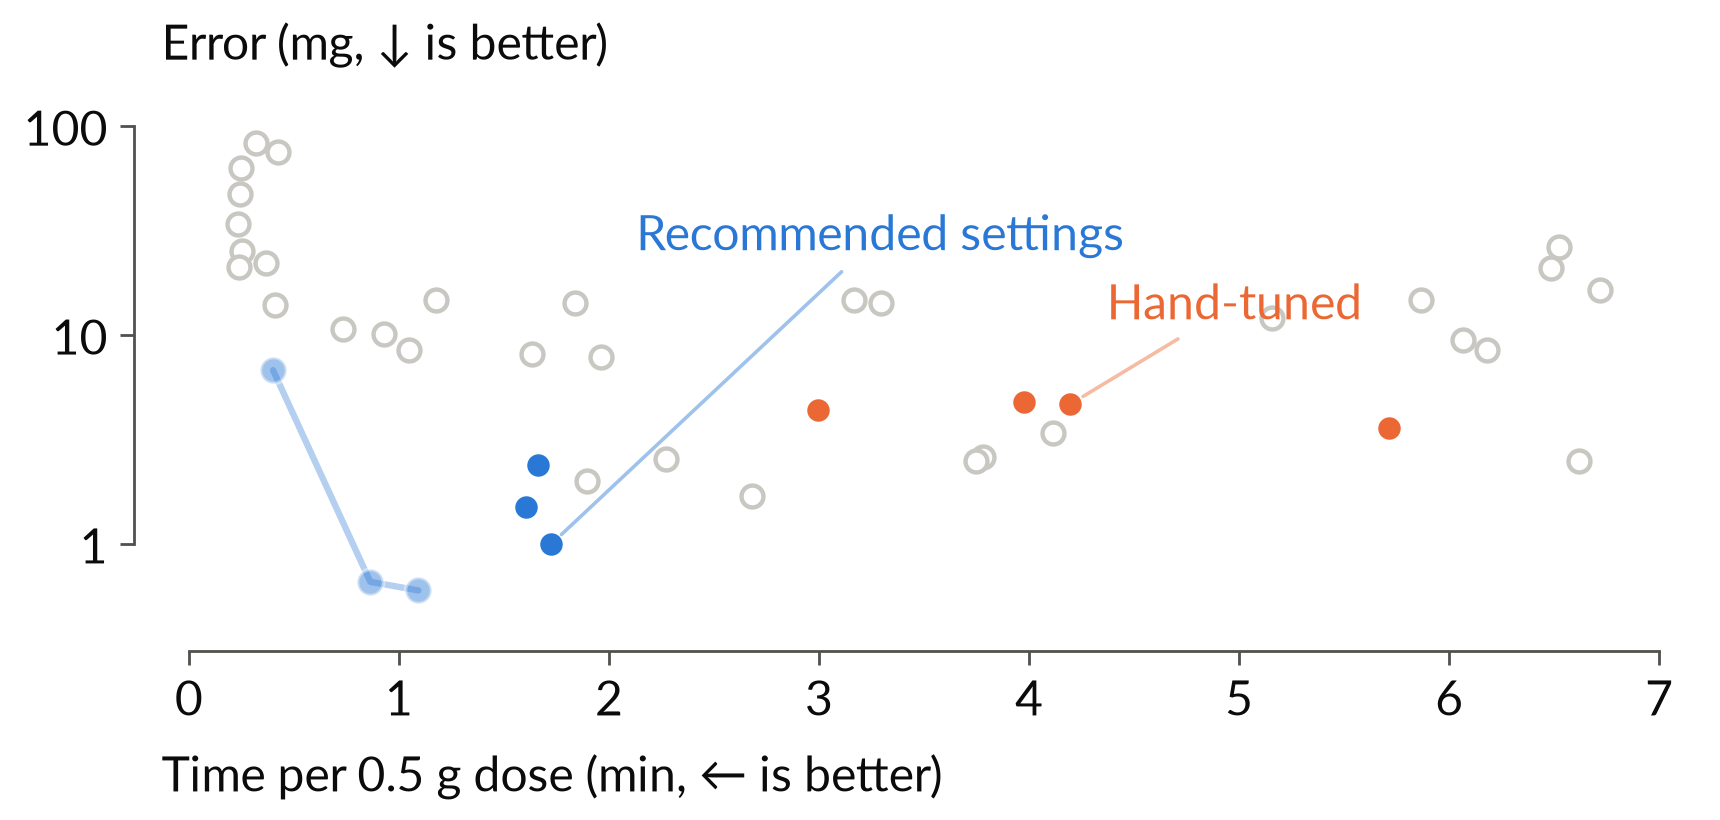
\includegraphics[width=\linewidth]{figures-cu-ded/doser-salt-pareto.png}
\end{minipage}\hfill
\begin{minipage}[c]{3.25in}
\caption{Bayesian optimization of the powder doser, on salt. Each gray
circle is one 0.5~g dose of the campaign, plotted by time and error. Light
blue joins the best single doses, blue marks doses at the recommended
settings, and orange marks hand-tuned settings.}
\label{fig:doser}
\end{minipage}
\end{figure}

% Fig. (CALPHAD): pycalphad-cu/run_calphad.py, MatCalc mc_ni v2.036 (ODbL).
\begin{figure}[t]
\centering
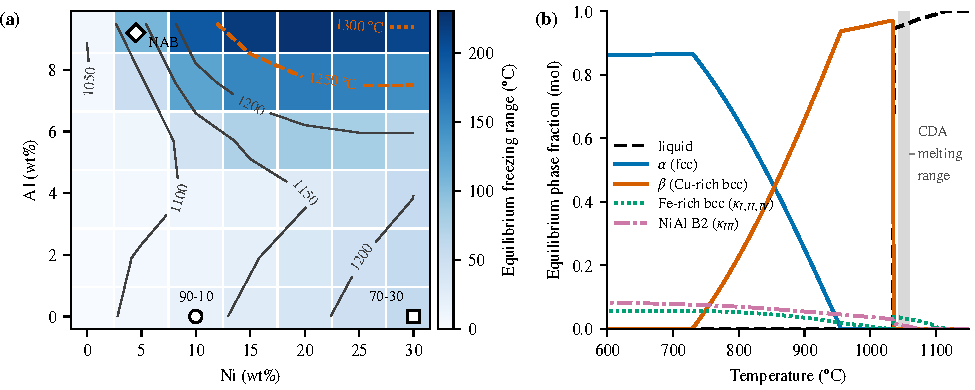
\includegraphics[width=\textwidth]{figures-cu-ded/cu_calphad_prelim.pdf}
\caption{pycalphad calculations with an open database, mc\_ni from
MatCalc~\cite{mcni}, which covers Cu-Ni-Al-Fe-Mn but was built for nickel
alloys. (a)~Equilibrium freezing range (color) and liquidus (contours,
\textdegree{}C) over the nickel and aluminum ranges of
Table~\ref{tab:space}, with 1~wt\% iron. Orange lines mark the
1,250\,\textdegree{}C liquidus cap and the 1,300\,\textdegree{}C limit of the
atomizer, and symbols mark the reference alloys. Values in the high-nickel,
high-aluminum corner are upper bounds. (b)~Equilibrium phase fractions of NAB
(C95800) against temperature. The gray band is the handbook melting
range~\cite{cdadata}.}
\label{fig:calphad}
\end{figure}

% Fig. 2 redraws the synthetic network from the MS&T26 talk
% (benchmarks/bofn-prelim/explain/frames/00-network.png); functions and costs
% are in benchmarks/bofn-prelim/README.md. It is the aluminum network, kept
% as is: it tests the method, not the alloy.
\begin{figure}[t]
\centering
\resizebox{\textwidth}{!}{%
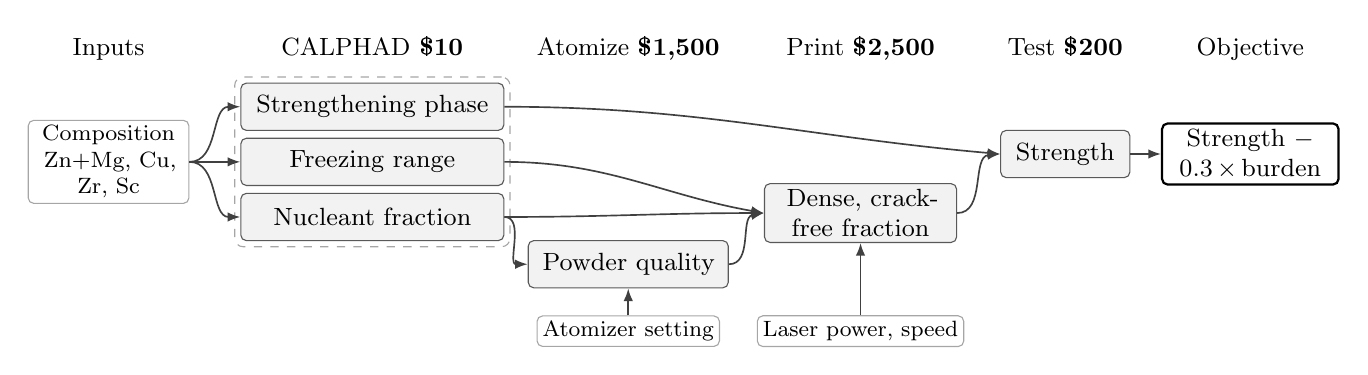
\begin{tikzpicture}[
  font=\small,
  nd/.style={draw=black!65, rounded corners=2pt, fill=black!5, align=center,
    minimum height=0.6cm, inner sep=2pt},
  inp/.style={draw=black!35, rounded corners=2pt, align=center,
    font=\footnotesize, inner sep=2pt},
  hd/.style={font=\small, anchor=base},
  e/.style={-{Latex[length=1.6mm]}, black!75, semithick}
]
\foreach \x/\t in {0.95/Inputs, 4.3/{CALPHAD \textbf{\$10}},
  7.55/{Atomize \textbf{\$1,500}}, 10.5/{Print \textbf{\$2,500}},
  13.1/{Test \textbf{\$200}}, 15.45/Objective}
  \node[hd] at (\x,2.75) {\t};
\node[inp, text width=1.9cm] (c) at (0.95,1.4) {Composition\\Zn+Mg, Cu,\\Zr, Sc};
\node[nd, text width=3.2cm] (s) at (4.3,2.1) {Strengthening phase};
\node[nd, text width=3.2cm] (f) at (4.3,1.4) {Freezing range};
\node[nd, text width=3.2cm] (g) at (4.3,0.7) {Nucleant fraction};
\node[draw=black!35, dashed, rounded corners=3pt, inner sep=2pt,
  fit=(s)(f)(g)] {};
\node[nd, text width=2.4cm] (q) at (7.55,0.1) {Powder quality};
\node[nd, text width=2.3cm] (r) at (10.5,0.75) {Dense, crack-\\free fraction};
\node[nd, text width=1.5cm] (u) at (13.1,1.5) {Strength};
\node[nd, draw=black, thick, fill=white, text width=2.1cm] (o) at (15.45,1.5)
  {Strength $-$\\0.3\,$\times$\,burden};
\node[inp] (a) at (7.55,-0.75) {Atomizer setting};
\node[inp] (l) at (10.5,-0.75) {Laser power, speed};
\foreach \n in {s,f,g} \draw[e] (c.east) to[out=0, in=180] (\n.west);
\draw[e] (s.east) to[out=0, in=175] (u.west);
\draw[e] (f.east) to[out=0, in=170] (r.west);
\draw[e] (g.east) to[out=0, in=180] (r.west);
\draw[e] (g.east) to[out=0, in=180] (q.west);
\draw[e] (q.east) to[out=0, in=190] (r.west);
\draw[e] (r.east) to[out=0, in=185] (u.west);
\draw[e] (u) -- (o);
\draw[e] (a) -- (q);
\draw[e] (l) -- (r);
\end{tikzpicture}}
\caption{Synthetic workflow used for Fig.~\ref{fig:sim}, built for the
aluminum version of this workflow: a hand-written function for each box and
a rough total cost (time, materials, supplies) for each step. Burden is a
penalty on scarce elements such as scandium. The nucleant (Zr, Sc) cuts
cracking, an effect the CALPHAD crack screen does not see. Task~1 replaces
these functions with copper and DED ones.}
\label{fig:synth}
\end{figure}

% Results: benchmarks/bofn-prelim/README.md (kappa = 1 headline, 20 seeds).
\begin{figure}[t]
\centering
\begin{minipage}[c]{3.1in}
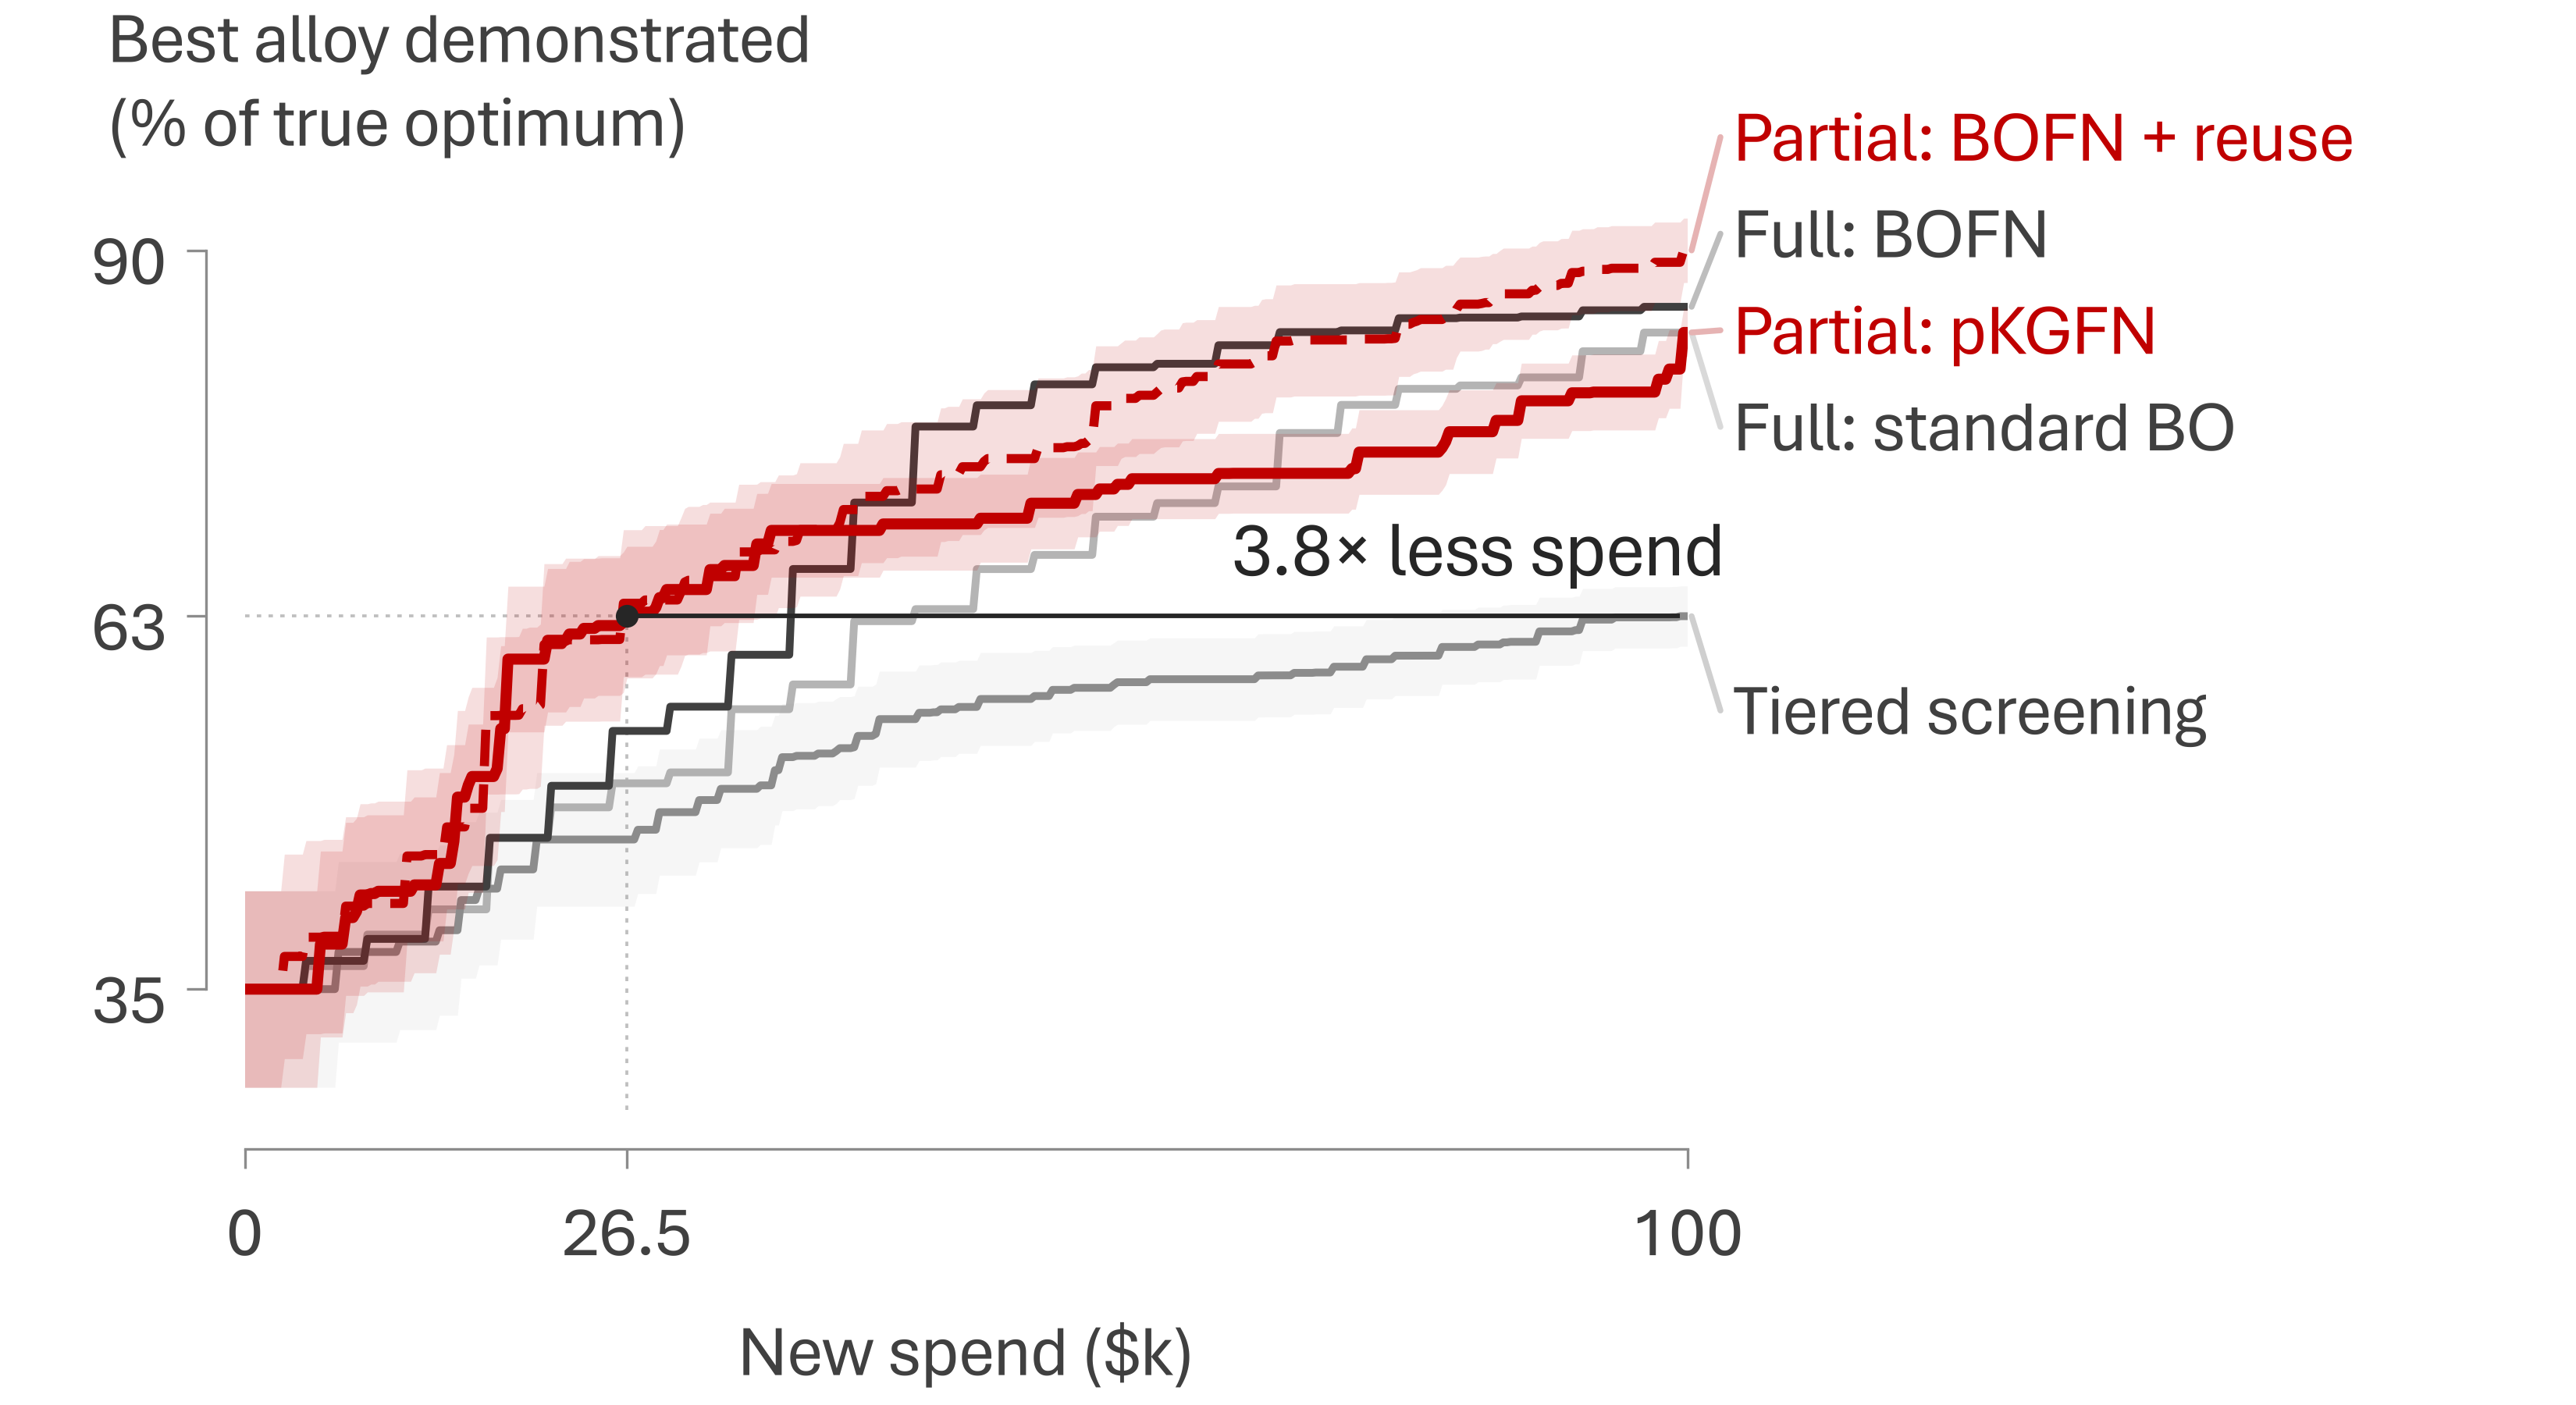
\includegraphics[width=\linewidth]{../../benchmarks/bofn-prelim/bofn_best_vs_spend_k1_partial_vs_full.png}
\end{minipage}\hfill
\begin{minipage}[c]{3.25in}
\caption{Best result found versus spend in simulations where the CALPHAD
crack screen ignores zirconium (means of 20 campaigns, $\pm$1 standard
error). Red searches choose the next step. Gray ones follow a fixed order.
pKGFN is the cost-aware method~\cite{buathong2024} and BOFN the linked-model
method~\cite{astudillo2021}. Reuse reprints earlier powders.}
\label{fig:sim}
\end{minipage}
\end{figure}

We also simulated the cost-aware method on a synthetic version of the
workflow (Figs.~\ref{fig:synth} and~\ref{fig:sim}), made for the aluminum
work. With the crack screen ignoring zirconium, screening
and then tuning the process stalled at 63\% of the optimum after \$100,000.
The cost-aware search, and a simpler one that reused powders, reached that
level after about \$26,500 (3.8 times less spend; 90\% confidence interval
2.0 to 5.7). Searches that ran every candidate through the full chain caught
up later, and screening kept pace when its physics was right. The simulation
is hand-built and has no measurement noise, with one objective, no corrosion branch, no
process physics, and one experiment at a time, so it does not test the
advances proposed here. It does show that letting the search choose the step
can pay off when the physics model is incomplete. The DED workflow
has the same structure: a physics screen that can miss effects, a powder
step, a deposition step, and tests.

\subsection{Method advances}

\subsubsection{Advance 1: several competing objectives}
The published cost-aware method optimizes a single objective. A copper alloy
for DED repair must balance deposit quality (dense, crack-free, and sound at
the fusion line with the part it repairs), strength, ductility, and corrosion
resistance in seawater, with no weighting known in advance. We will extend
the cost-aware rule to several objectives. We will replace the expected
improvement in one objective with the expected growth of the set of best
trade-offs (the Pareto front), divided by cost as before. That growth is
measured by the volume of property space that the trade-offs
outperform~\cite{daulton2021}. The difficulty is that each cheap measurement informs some objectives strongly
and others weakly. Single tracks show cracking and dilution well but say
little about strength or corrosion, and a polarization measurement says much
about corrosion rate and nothing about strength. The rule has to account for
that through the network. We will derive the rule, check it against
exhaustive calculations on small problems, and measure its computing time on
BYU high-performance computing.

\subsubsection{Advance 2: results that arrive out of order}
The published method chooses one experiment at a time and waits for its
result. In this workflow a DED session deposits many specimens, microscopy
results arrive days later, immersion tests run for weeks, and thermodynamic
calculations finish in minutes. We will extend the rule to groups of experiments
whose results arrive at different times, so that new experiments are chosen
while others are still running. Experiments in progress will enter the models
as stand-in results drawn from the current predictions, a standard way to
avoid choosing the same experiment twice~\cite{snoek2012}. We will also test how
stable the choices are when a late result contradicts early ones. For
example, a block that looked dense on its surface may show cracks under the
microscope, or an alloy that passed the polarization screen may show
selective attack after a month of immersion.

\subsubsection{Advance 3: physics computed for the process}
Standard CALPHAD inputs describe equilibrium, or solidification without
diffusion in the solid, and ignore the thermal history of the
process~\cite{debroy2018}. We will add inputs computed along the DED thermal
history (Section~\ref{sec:concepts}): cooling rate through solidification, the peak
temperatures of reheating, and the phases that CALPHAD allows at those
temperatures. Hypothesis H3 tests whether these inputs make the models'
predictions more reliable than equilibrium inputs, and whether equilibrium
inputs beat data alone. The answer measures what incomplete, process-aware
physics is worth inside a search, which sets how much simulation a campaign
should buy before it buys experiments.

\subsubsection{Advance 4: a physical workflow from powder to repair}
We will demonstrate the advances on a physical workflow (Fig.~\ref{fig:network})
in which the search chooses the composition, the atomizer settings, and the
deposition settings, and decides at each step whether a candidate goes on.
After microscopy, specimens go to tensile tests, or to the corrosion screen
and, for selected candidates, to immersion tests. Candidates that deposit well
get a repair coupon: a deposit on cast NAB or wrought copper-nickel plate,
checked for cracks, dilution, and hardness across the fusion line. These
checks do not show whether a repair will last. Crack growth in printed
steels varies with the build process~\cite{jones2026}, so fatigue and
residual stress of repairs are left to Navy laboratories.
Pre-placed tracks on the same plates, at Utah, come first. The
demonstration includes real deposit-to-deposit scatter, outputs computed from
microscopy images, and three inputs that enter at different steps.

\subsubsection{Advance 5: checking what the screens discard}
A cheap screen saves money only if it does not discard good candidates, and
Section~\ref{sec:naval-cu} shows that a short corrosion screen can also pass
bad ones. Each round, the search will send a small random share of the
candidates it would stop, about one in ten, on to the next step anyway. These
audited candidates measure how often each screen is wrong, and they keep the
models from learning only from candidates that the screens favored.

\subsection{Hypotheses and rejection criteria}

\textbf{H1 (cost).} The cost-aware search, with several objectives and
experiments in progress, will reach a target set of trade-offs at lower
total cost than standard Bayesian optimization with several objectives,
which carries every candidate through the full chain. H1 will be rejected if, across
matched campaigns with the same budget, the median cost to reach the target is
not lower than that of the full-chain baseline.

\textbf{H2 (calibration).} The predicted probabilities that a candidate will
deposit dense and crack-free, fuse to the repair substrate without cracks,
and stay close to its intended composition will match the observed rates on
deposits the models have not seen. H2 will be rejected if observed success rates differ from
predicted probabilities by more than 10 percentage points.

\textbf{H3 (process-aware physics).} CALPHAD outputs evaluated along the DED
thermal history will improve that calibration over CALPHAD outputs at
equilibrium, which will in turn improve it over models trained on data
alone. H3 will be rejected if the process-aware inputs do not reduce
calibration error on unseen deposits compared with the equilibrium inputs.

\textbf{H4 (pending results).} Choosing new experiments while others are
pending will reach the target in less calendar time than waiting for each
batch to finish, at equal spend. H4 will be rejected if, in median calendar
time, the version that works around pending results is no faster than the
version that waits.

\textbf{H5 (corrosion screen).} Corrosion rates, breakdown potentials, and
impedance from the one-hour screen, together with composition and
microstructure, will predict which candidates pass a 30-day immersion test.
To pass, a candidate needs a mass loss no greater than that of the 70-30
copper-nickel reference and selective attack no deeper than \todo{depth. Immersions of 21 and 30 days in salt
solution found at most 1.8 to 3.4~$\mu$m in laser-deposited NAB~\cite{zhao2022}
and more than 3~$\mu$m in cast NAB~\cite{tan2024}. Options: a few micrometers, or
no deeper than in the cast NAB reference}. H5 will be
rejected if, among tested candidates (audited ones included), those that the
model ranks in the top half pass no more often than those in the bottom half.
We will also report the rank agreement of screen and immersion and the share
of passing candidates that the screen rejects, with confidence intervals, and
will test a few candidates just either side of the cutoff.

We will fix and post the targets, baselines, budgets, and number of matched
campaigns before each test starts \todo{confirm a public
pre-registration site, e.g., OSF}. We test H1 and H4 first on simulated
benchmarks and on benchmarks built from past data, where many matched
campaigns are affordable, and
then in live campaigns, where only a few are.

\subsection{Research plan}

\subsubsection{Task 1: methods (Ph.D. student 1)}
Derive and implement the rule for several objectives (Advance 1), the rule for
pending results (Advance 2), the process-aware physics inputs (Advance 3),
and the audit of screened-out candidates (Advance 5). Build simulated
benchmarks that replace the functions of Fig.~\ref{fig:synth} with copper and
DED ones, with noise, several objectives, a corrosion branch, and delays
drawn from measured turnaround times. Build benchmarks from past data: our
aluminum data and the copper data that Task 2 adds each year.

\subsubsection{Task 2: experimental platform (Ph.D. student 2)}
\label{sec:task2}
We will make powder for each candidate in our laboratory. Oxygen-free copper
bar is machined into cups that hold the charge. We weigh in nickel, iron,
manganese, aluminum, and other additions to 0.1~mg as pure metals or copper
master alloys. A charge is about 0.5~kg, as in the published CuSn8
runs~\cite{choma2026} \todo{confirm the charge size after the first copper
runs}. Minor additions that come as powder are dispensed into the cup by our
powder doser (Section~\ref{sec:prelim}), which weighs and logs each dose, so every lot carries a record of what went into it. The charge is
melted in a graphite
crucible in the induction module of the ultrasonic atomizer (AMAZEMET
rePOWDER) and poured through a 0.5~mm nozzle onto a vibrating plate, where it
breaks into droplets. Nickel and iron react with graphite. Before melts that
contain them, we spray the crucible with a thin boron nitride coating, which
lasts a few runs, and pour through a boron nitride nozzle, as the
manufacturer advises. NAB has already been atomized from a
graphite crucible on a rePOWDER~\cite{muller2023}. Many alloys wet bare carbon-carbon
composite poorly~\cite{choma2026}, so the plate is carbon-carbon with a
molybdenum- or tungsten-based coating where the melt lands. The first part of
each pour heats the plate until the melt wets it, and atomization is then
continuous. With such plates on our model of atomizer, the manufacturer
turned 80 to 90\% of each charge of a tin bronze (CuSn8) into
powder~\cite{choma2026}. \todo{confirm with AMAZEMET the plate and nozzle
for NAB and copper-nickel; the published NAB runs used a bare carbon-fiber
plate that left fibers in the powder~\cite{uhlmann2024}}. The median droplet
size follows the wavelength of capillary waves on the plate, so it falls as
the frequency to the power $-2/3$~\cite{lang1962}. The plates on our unit vibrate
at 40~kHz, where the Lang relation gives a median near 47~$\mu$m for a copper
melt. Measured powders are coarser. NAB atomized at 40~kHz had a median of
98~$\mu$m~\cite{uhlmann2024}, about twice that estimate, and much
of the CuSn8 powder made at 40~kHz on our model fell between 63 and
150~$\mu$m~\cite{choma2026}. Both suit the DED system described below,
which takes powder of about 50 to 150~$\mu$m, sometimes up to 200~$\mu$m, and
is usually fed cuts of 45 to 105 or 100 to 200~$\mu$m. Published blown-powder
work on bronzes used 45 to 106 and 45 to 150~$\mu$m
cuts~\cite{li2021,pi2025}. We sieve each lot into those two cuts. We check its
size distribution (sieve analysis and SEM images), flow and apparent density
with a Hall funnel~\cite{astmB213,astmB212}, shape, satellites, and stray
plate fibers (SEM), and oxygen and carbon content. \todo{name the service
laboratory: inert-gas fusion for oxygen, combustion for carbon}. Powder
oxygen also matters at a repair. In a model system, additions whose oxides
are more stable than that of the parent metal improved wetting and bonded
area~\cite{fisher2019}, so the models relate the oxygen of each lot to fusion
on cast NAB and wrought copper-nickel. The atomizer settings
the search chooses are the melt temperature, the pour pressures, and the
plate amplitude, and the share of each lot in each cut is an output of the
powder step. With the gas flows and the laser spot, the size distribution sets
how much of the powder the melt pool catches~\cite{ancalmo2025}. The search chooses the atomizer settings along with the
composition, so the powder, not only the alloy, is designed for blown powder.

We buy DED as machine time at two facilities, and the search treats them as
two steps of different cost (Fig.~\ref{fig:network}). Neither facility is a
subawardee. For the small step we use an InssTek MX-Lab at the University
of Utah,
in the laboratory of Professor Z.~Zak Fang, 45 miles from BYU, which his
group has offered to the project. It has a 500~W fiber laser, 150~mm of travel on each
axis, control of melt-pool height, and six powder feeders that can each be
run separately~\cite{insstek,utahded}. \todo{confirm with Fang: the rate, the
smallest powder charge per feeder, the argon chamber and any preheat, and
that a BYU student runs it after training}. We start every composition here.
We spread powder from a first lot in grooves machined in plates, including
cast NAB and wrought copper-nickel plate, and melt it at several laser powers
and speeds. These pre-placed tracks use a few grams of powder each and show
cracking, porosity, dilution, and fusion to the repair substrates. They
differ from blown-powder tracks in heat input and in how the powder reaches
the melt pool, so the models treat them as a cheaper, less faithful
measurement. Once its tracks are sound, a composition gets blown-powder
deposits from one 0.5~kg lot. Single tracks at several laser powers, travel
speeds, and powder feed rates show melt-pool size, dilution, cracking, and
the share of the powder caught in the melt pool. Thin walls show cracking
and heat buildup, and small blocks show density and porosity. The heat flow model is
calibrated separately for each kind of track, and the audit of Advance~5
measures how often the tracks mislead.

For the large step we buy sessions on a FormAlloy X2 blown-powder laser DED
system at the Colorado School of Mines, run by facility staff at its external rates for
machine time and labor. Facility staff plan 3~hours of machine time and
2~hours of labor for a typical session of four 25~mm cubes. Mines plans on
the melt pool catching about half the powder fed, and needs about 2~kg of
each powder to fill the hoppers of the X2. Since 2~kg takes about six
atomizer runs, only compositions whose small blocks at Utah reach 99\%
relative density are scaled up. Their sessions at Mines build blocks for
sub-size tensile bars (ASTM E8/E8M) and corrosion coupons at the chosen
settings. They also build repair coupons on thick cast NAB and wrought
copper-nickel plate (Advance~4), where fusing the first layer to a large
heat sink needs more laser power than the MX-Lab has. \todo{confirm the X2's laser (wavelength, power, spot size), its
shielding, substrate preheat, turnaround, and that powder left in the hopper
comes back to us}. Commercial 70-30 copper-nickel and NAB powders, deposited
at both facilities, are the baselines \todo{confirm commercial powder
sources, at least 2~kg of each; Mines can also supply powder at cost}. The
search decides which compositions go to Mines at all.

At BYU we will examine selected deposits by SEM, and by EDS and inductively
coupled plasma mass spectrometry for composition, since manganese and
aluminum can be lost to evaporation and oxidation~\cite{debroy2018}.
Electron backscatter diffraction (EBSD) gives grain size, texture, and phase
fractions, including martensitic $\beta'$ in the bronzes. Finalists also get
transmission electron microscopy, so that fine $\kappa$ precipitates, which
SEM can miss, are measured rather than assumed. Replicate tracks and blocks at
fixed settings will measure deposit-to-deposit scatter. Image analysis
scripts will turn micrographs into porosity, crack length, dilution, grain
size, and phase fractions with stated uncertainty.

Corrosion tests follow the same staging. The screen runs on the
liquid-handling gantry in our laboratory (CubXL, Ursa Laboratories), which is
already driven by scripts, so the search can schedule it like any other
step. The gantry fills small O-ring wells, 3 to 4~mm across, clamped on
polished faces, with substitute ocean water~\cite{astmD1141}, and a
potentiostat dedicated to the loop measures open-circuit potential, linear
polarization, impedance, and cyclic polarization~\cite{astmG59,astmG61}.
Small cells can add crevice attack at the seal and shift breakdown
potentials~\cite{frankel1998}. We therefore photograph each spot before and
after and check the wells against a conventional 1~cm$^2$ flat cell on the
references. \todo{choose the potentiostat: a module unit with
impedance on the gantry, cross-checked on a borrowed laboratory instrument,
or the benchtop unit and flat cell in Field 11; see cubxl-electrochemistry.md}.
Several wells fit on one specimen, so a repair coupon is measured in the
deposit, at the fusion line, and in the heat-affected zone of the substrate,
where welded NAB was attacked selectively~\cite{dobson2024}.
The gantry then pipettes the used electrolyte of each well into a tube for
inductively coupled plasma mass spectrometry, which shows which elements
left the surface, for example aluminum from NAB or nickel from
copper-nickel. ASTM G61 is written for \mbox{iron-}, \mbox{nickel-}, and
cobalt-based alloys, so we will report how its procedure behaves on
deposited copper alloys. We measure wrought 70-30 copper-nickel and
heat-treated cast NAB as references in every round. The screen is a ranking
that has to be calibrated, so deposits and references get the same
preparation and exposure, in replicate, and the conditions that control
seawater tests are recorded~\cite{shifler2002,shifler2022}. Candidates that the
search selects get 30-day immersion tests in capped vials on the deck of the
gantry. The gantry draws a few microliters of each solution at about 1, 3,
10, and 30 days for the same analysis. The metal released over time then
enters the models as an intermediate result between the one-hour screen and
the final mass loss. We weigh the coupons before and
after~\cite{astmG31,astmG1} and section them to find the deepest selective
attack. Repair coupons are also immersed whole, with a stated ratio of
deposit to substrate area, because a repair is a galvanic
couple~\cite{shifler2006}. Simulated pits in printed microstructures grow
deeper than in a uniform model~\cite{brewick2022}, and crevice damage in
printed stainless steel, measured in three dimensions, has tracked the
electrochemistry~\cite{hangarter2025}. Microstructure therefore stays in the
corrosion model. The leading candidates get crevice and longer immersion tests \todo{confirm the
durations, and natural or substitute seawater}. Tests in flowing seawater,
which take months, are left to Navy laboratories, such as the marine
corrosion laboratories at NSWC Carderock~\cite{carderockpartner}, for the
three leading candidates and the two references \todo{confirm the number
with Carderock} (Section~\ref{sec:naval}).

We chose the search space the way we chose our aluminum palette: a
literature review of each candidate element, then a check of its coverage in
the CALPHAD database. We reviewed fifty elements from the periodic table one
at a time. They include every element that appears in a commercial copper
alloy, a copper alloy or welding filler specification, a deoxidizing
practice, or the crucible and plate materials of the atomizer. Each review
asked four questions. Does the element help seawater resistance, deposit
soundness, or repair? What sets its upper limit? Can it be melted and
atomized below 1,300\,\textdegree{}C without attacking the crucible or
plate? Does the Thermo-Calc copper database
(TCCU7~\cite{tccu7}) assess its systems? We search eight elements from
the start (Table~\ref{tab:space}), with copper as the balance at no less
than 65\% and a calculated liquidus no higher than 1,250\,\textdegree{}C.
In Year~2 we will test zirconium and boron, tin and germanium in NAB, and
one rare earth, lanthanum or cerium, which improved a 90-10 alloy in salt
solution~\cite{du2025}. Rules tied to the aluminum content keep each candidate near
known metallurgy. Above 7\% aluminum, nickel must at least equal iron, as it
does in the nominal composition of Navy NAB castings~\cite{milb24480}. Below
1.5\%, iron stays at or
below 2.3\%, the upper limit of the iron-rich 70-30 grade C71640, so that it
remains in solid solution~\cite{astmB111}. Chromium and niobium are used only
where aluminum is at most 3\%, and silicon above 0.1\% only with niobium, as
in cast 70-30 copper-nickel~\cite{astmB369}. Retained $\beta$ is not limited
by a fixed formula. The process-aware CALPHAD inputs predict it
(Advance~3). The space includes the region between the two families,
copper-nickel-aluminum alloys such as the high-strength
MARINEL~\cite{campbell2002}, where low-nickel candidates may lie. Beryllium
and cadmium (toxic powder and fume), zinc (it evaporates in the melt pool and
dezincifies in seawater), and the refractory metals (immiscible, and far
above the melting limit) are excluded. Lead, sulfur, phosphorus, carbon,
bismuth, and the other impurities are held at or below the welding-grade
limits for copper-nickel~\cite{awsA57}. All the searched elements but iron
are on the 2025 U.S. list of critical minerals~\cite{usgs2025}. Nickel
dominates by mass and is carried as an objective.

\begin{table}[h]
\centering
\caption{Elements searched from the start (wt\%), with copper as the balance
(at least 65\%) and a calculated liquidus of at most
1,250\,\textdegree{}C. ``Cu-Ni only'': used where aluminum is at most 3\%
(silicon: below 7\%).}
\label{tab:space}
\renewcommand{\arraystretch}{1.1}
\begin{tabularx}{\textwidth}{@{}l l >{\raggedright\arraybackslash}X >{\raggedright\arraybackslash}X@{}}
\toprule
\textbf{Element} & \textbf{Range} & \textbf{Role} & \textbf{Upper limit set by} \\
\midrule
Ni & 0--30 & Protective film in Cu-Ni; $\kappa$ phases in NAB & Liquidus near
  the atomizer's limit; supply (an objective) \\
Al & 0--9.5 & Aluminum bronze; Cu-Ni-Al alloys & Retained $\beta'$
  martensite as deposited \\
Fe & 0--4.5 & Film in Cu-Ni; $\kappa$ phases in NAB & Iron out of solution in
  Cu-Ni; coarse $\kappa$ in NAB \\
Mn & 0--4 & Deoxidizer; partial nickel substitute & Evaporation and
  oxidation in melting and DED \\
Cr & 0--0.7, Cu-Ni only & Resistance to fast flow~\cite{lewis1981} & Cr-rich
  particles; crevice attack in still water \\
Si & 0--0.5, Cu-Ni only & Deoxidizer; strength with Nb & Silicides; weld
  cracking \\
Nb & 0--0.8, Cu-Ni only & Weldability of cast Cu-Ni & Undissolved Nb-rich
  particles \\
Ti & 0--0.5 & Deoxidizer in Cu-Ni welding filler~\cite{awsA57} & Oxide and
  nitride inclusions; crucible attack \\
\bottomrule
\end{tabularx}
\end{table}

\subsubsection{Task 3: live campaigns and hypothesis tests (both students)}
Run live campaigns in which the search chooses each experiment and step.
The campaigns are supervised by people, who book the DED sessions and handle
the coupons. Compare the search on equal budgets with random selection, with
a fixed funnel that passes the top candidates at each step, and with standard
Bayesian optimization with several objectives over the full chain. Versions
that drop the costs or the physics inputs show what each adds. A funnel that
looks sensible can do worse than random selection~\cite{reyes2022}. Score each on total dollars and DED hours to a
confirmed candidate. Report the false rejections at each step, the
calibration at each link, and the error on compositions outside the
training family, such as NAB predicted from copper-nickel data. We test the
transfer of results from the Utah system to Mines on paired compositions, as
has been done between wire and powder DED~\cite{huang2026}. Test H2
and H3 on unseen deposits, H5 on the audited and selected candidates, and H1
and H4 in matched campaigns.

\subsubsection{Task 4: release and transition}
Release the software, data, and models each year (Section~\ref{sec:dmp}).
Write a short guide for applying the method to other alloys, deposition
processes, and test sequences, aimed at Navy laboratory and depot engineers.
The search narrows the field. Each finalist then gets replicated builds and
a dataset in the form of the Carderock property
databases~\cite{norkett2025,orzolek2023}: powder specification, deposition
settings, and tensile, corrosion, and repair-coupon data, with the raw files
public. We share them with materials engineers at NSWC Carderock, who can
decide which candidates merit flowing-seawater and service tests. The
finalists will be candidates for Navy qualification testing. Component tests, fatigue, inspection methods, and design allowables
would remain, as would the decision whether a controlled repair consumable
or a revision of a specification such as MIL-PRF-32816~\cite{milprf32816} is
warranted.

\subsection{Expected results and new knowledge}

If successful, the project will produce:
\begin{enumerate}\setlength{\itemsep}{0pt}
\item The first cost-aware method of this kind for competing properties and
staggered results.
\item A measured answer to how much a staged, cost-aware search saves over
full-chain testing on a real alloy workflow.
\item A measured value of process-aware physics: how much CALPHAD evaluated
along the DED thermal history improves predictions over equilibrium
calculations and over data alone.
\item Corrosion data for copper alloys deposited by DED, and a measured link
between a one-hour electrochemical screen and immersion tests that take
weeks.
\item New copper alloy compositions designed for blown-powder DED, each with
its powder specification, deposition settings, tensile properties, corrosion
behavior, and repair coupons, using less nickel where the trade-offs allow.
\end{enumerate}
Results that reject a hypothesis are also new knowledge. For example, if H1
fails, the data will show the step whose cost or noise erased the advantage.
If H3 fails, they will show which process effects the calculations missed. If
H5 fails, they will show which microstructural features the screen missed.

\subsection{Future Naval Relevance}
\label{sec:naval}

\textbf{ONR S\&T Focus Areas.} The primary focus area is Manufacturing,
research area Integrated Manufacturing and Sustainment Technologies. The
secondary focus area is Materials and Electronics, research area Sustainable
and Operationally Robust Materials. Within Code 332 the project fits the
program Materials \& Processes for Additive Manufacturing~\cite{onram}. That
program lists five thrusts: ``(i) rapid qualification frameworks; (ii)
tailored AM materials and processes; (iii) large scale AM; (iv) additive
repair and (v) AM and digital logistics''~\cite{onram}. Its research
challenges include
to ``develop and validate computational approaches for AM materials and
processes for engineering applications'' and to ``develop large-scale AM
processes for naval materials of interest''~\cite{onram}. The project serves
thrusts (ii) to (iv) with an alloy designed for a large-scale process that
also repairs, and thrust (i) with a search method that decides which test to
run next and states its confidence in the outcome. It is ICME for additive
manufacturing, the approach that the ONR Structural Metals program calls ``an
efficient rigorous framework for optimizing processing and manufacturing
schemes''~\cite{onrsm}: computation first, and experiments where they change
a decision. It also fits two other Code 332 programs. Corrosion Science and
Corrosion Control Technologies asks for a ``fundamental understanding of
corrosion mechanism in additive manufactured (AM) alloys''~\cite{onrcorr}.
The thrusts of Computer-Aided Materials Design include high-throughput
screening concepts and informatics~\cite{onrcamd}.

\textbf{Copper alloys, castings, and repair.} The slow production of large
castings ``has historically gated progress and throughput for both the
Columbia and Virginia submarine programs''~\cite{navsup2026}, and the Navy is
replacing castings with printed parts. In August 2026 it set out ``a
streamlined, repeatable technical pathway to substitute legacy cast and
wrought parts with 3D-printed metallic materials''~\cite{navy2026ppd}. A
printed copper-nickel deck drain, made ``to provide an alternative to
traditional copper-nickel castings,'' has been installed on a
new-construction submarine~\cite{hii2023,nns2025}, and the Navy Maritime
Industrial Base program has made copper-nickel ship-service ball valves by
wire-arc deposition~\cite{dvids2025}. These parts use the cast compositions,
as does ONR-funded research on wire-arc 70-30 copper-nickel~\cite{song2024}.
A copper alloy designed for blown-powder DED, one that resists seawater as
deposited, would let a shipyard or depot build a part that now waits on a
casting. It would also let them restore a worn part in place without the
heat treatment the cast alloys need. The ONR corrosion program asks for this
kind of work: ``modify the
chemistry of feed stock materials to enhance AM processing and corrosion
resistance of additive-manufactured alloys''~\cite{onrcorr}.

\textbf{The longer horizon.} The project designs for single-stream,
pre-alloyed powder, which existing DED systems can use now. The same models
can later choose blends of elemental and master-alloy powders fed from
several hoppers and alloyed in the melt pool, which would let a depot make a
new composition without a new powder lot. The guide of Task~4 will describe
that extension. The method needs only a network of steps, their costs, and
their measurements, so it also applies to wire-arc and laser-wire deposition
and to other Navy alloys, including titanium. A plasma melting module for our
atomizer (not part of this request) would extend the powder work to alloys
that melt above the limit of the induction module.

\textbf{Navy engagement and people.} The Naval Surface Warfare Center
(NSWC) Carderock Division is the Navy lead for additive manufacturing
technology and the NAVSEA lead for welding process and material
specifications~\cite{carderocksm}, and it runs marine corrosion
laboratories~\cite{carderockpartner}. Its engineers have studied how
processing sets the microstructure of NAB~\cite{orzolek2022} and published
the temperature-dependent properties of copper-nickel and wire-arc NAB that
our heat flow model uses~\cite{norkett2025,norkett2026a,norkett2026b}.
The PI presented autonomous experimentation for alloy discovery at Carderock
on 14 October 2026, hosted by
Dr.~Nicholas J.~Jones, to an audience of 54 \todo{name any Carderock
contacts who agree to be listed, and confirm Dr.~Jones's title and code}.
Each year we will send the candidates and data to materials and corrosion
engineers at Carderock and ask them which flowing-seawater and repair tests
the final candidates should get. We will visit in Years~2 and~3 (both trips
are in the budget). The PI will apply to the Summer Faculty Research Program to
spend a summer at Carderock \todo{confirm; the 2027 application closes
14 December 2026; Carderock's SFRP topics include sustainment, repair, and
corrosion science}. The project will train two Ph.D.\
students and undergraduates in powder making, deposition,
characterization, corrosion testing, and autonomous experimentation.
Undergraduates join from our research group and from the courses the PI
teaches \todo{name the courses}. We will
encourage them to apply to the Naval Research Enterprise Internship Program
and the SMART and NDSEG programs, which the NOFO names as goals of the YIP.

\subsection{Project Schedule and Milestones}

Table~\ref{tab:schedule} lists the schedule by year. The award start date is
1 April 2027.

\begin{table}[h]
\centering
\caption{Schedule and milestones (Y = project year, starting 1 April 2027).}
\label{tab:schedule}
\renewcommand{\arraystretch}{1.15}
\begin{tabularx}{\textwidth}{@{}p{0.4in}>{\raggedright\arraybackslash}X>{\raggedright\arraybackslash}p{2.05in}@{}}
\toprule
\textbf{Year} & \textbf{Work} & \textbf{Milestone (month)} \\
\midrule
Y1 & Derive the rule for several objectives; build simulated benchmarks and
benchmarks from past data; build the process-aware physics inputs; first copper powder lots
in the DED size range and their tracks at Utah; deposit the commercial
baselines at both facilities and replicate them to measure scatter; set up the corrosion screen on wrought and cast references;
automate image analysis. & M1: first copper powder lot sieved, checked, and
melted in tracks at Utah (4).\newline M2: baseline deposits and scatter measured (7).\newline M3:
corrosion screen repeatability measured (8).\newline M4: rule for several objectives
passes small-problem checks (9).\newline M5: benchmarks frozen and posted
(12). \\
Y2 & Derive the rule for pending results; first live campaign with tensile,
corrosion, and repair branches; first 30-day immersions; test H2 and H3 on
unseen deposits. & M6: first live campaign done (18).\newline M7: H2 and H3
tested (22).\newline M8: methods paper and software release 1 (24). \\
Y3 & Matched live campaigns against the full-chain baseline; test H1, H4, and
H5; release software, data, and guide; share powder, deposition, corrosion,
and repair data with Navy engineers. & M9: matched campaigns done
(32).\newline M10: H1, H4, and H5 tested (34).\newline M11: final release and
report (36). \\
\bottomrule
\end{tabularx}
\end{table}

\subsection{Goals and Benchmarks}

Table~\ref{tab:goals} lists each goal and the benchmark used to measure
progress. Progress will be reported at each ONR program review.

\begin{table}[h]
\centering
\caption{Goals and the benchmarks that measure them.}
\label{tab:goals}
\renewcommand{\arraystretch}{1.15}
\begin{tabularx}{\textwidth}{@{}>{\raggedright\arraybackslash}p{1.75in}>{\raggedright\arraybackslash}X@{}}
\toprule
\textbf{Goal} & \textbf{Benchmark} \\
\midrule
Cost-aware rule for several objectives & Matches exhaustive calculations
on small problems; finds a larger set of trade-offs per dollar than a
full-chain search on the simulated benchmark. \\
Rule for pending results & Same final quality as the one-at-a-time rule in
less calendar time on the simulated benchmark with measured delays (H4). \\
Calibrated predictions & Observed success rates within 10 percentage points
of predicted probabilities on unseen deposits (H2). \\
Process-aware physics & Lower calibration error with thermal-history inputs
than with equilibrium inputs, and with equilibrium inputs than without (H3). \\
Powder for blown-powder DED & Every deposited composition made in-house,
sieved to the DED size range, with its size distribution, flow, and oxygen
and carbon content recorded. \\
Corrosion screen & Top-ranked candidates pass the 30-day immersion test
more often than bottom-ranked ones (H5). \\
Lower cost on real deposits & Lower median cost to reach the target than the
full-chain baseline in matched live campaigns (H1). \\
New alloys & At least \todo{number} new compositions deposited dense and
crack-free, with tensile, corrosion, and repair-coupon data, beyond the
commercial baselines. \\
Open release & Software, data, and models posted each year with tests and
documentation. \\
\bottomrule
\end{tabularx}
\end{table}

\subsection{Gold Standard Science}

Executive Order 14303 lists nine tenets of Gold Standard
Science~\cite{eo14303}. Such science is reproducible, transparent,
communicative of error and uncertainty, collaborative and interdisciplinary,
and skeptical of its findings and assumptions. It is also structured for
falsifiability of hypotheses, subject to unbiased peer review, accepting of
negative results as positive outcomes, and without conflicts of interest. The
plan follows each point. Each hypothesis above has a stated rejection
criterion, and we fix the targets and baselines before each test. Every
prediction carries an uncertainty, and the calibration tests (H2, H3) check
whether that uncertainty is honest. The random audit of Advance~5 tests the
assumptions behind each screen. Replicate deposits and
reference specimens measure scatter so that it is not mistaken for a real
effect. We release code, data, and models each year so others can rerun
every analysis. We will publish results that reject a hypothesis like any
other result. The record of the PI supports this: the PI co-authored a review of
self-driving laboratories and led open benchmark and software projects (see
Section~\ref{sec:quals}).

\section{Management Approach}
\label{sec:mgmt}

This is a single-PI project with no co-PIs or subawards. The PI will lead the
method development, set the campaign plans, and supervise all students.
Ph.D.\ student 1 will lead Task 1 (methods, physics inputs, benchmarks,
software). Ph.D.\ student 2 will lead Task 2 (powder, deposits, microscopy,
tensile and corrosion tests). An undergraduate researcher will help make and
check powder, prepare specimens, and run the corrosion screen. Both Ph.D.\
students share Task 3, so the methods are tested on the data they will face.

We buy DED time from the University of Utah and the Colorado School of
Mines, and any outside tests from a commercial laboratory. None is a
subaward. A BYU student runs the Utah sessions after training by the Utah
group, and staff at Mines run each session there. Both follow the settings
the search chooses. \todo{if Fang or Sam agrees to be named as an unfunded collaborator,
say so here and list them under current and pending support (NOFO p.~38)}.
Our budget buys about eight half-day sessions a year at Utah and 11, 13,
and 9 sessions at Mines in Years 1 to 3. \todo{the Utah line is an allowance
until Fang sets a rate; dropping the \$18,000 potentiostat (Field 11) would
buy about 14 more Mines sessions in Year~1}. All other work is at BYU: our
atomizer laboratory, the BYU Microscopy Center (SEM, EDS, EBSD), and
BYU high-performance computing. The team meets weekly to review new results and
choose the next experiments. A shared database records every step, so the
search always sees the latest results. The schedule and milestones are in
Table~\ref{tab:schedule}.

\textbf{Risks and responses.} If the rule for several objectives is too slow to
compute, we will use a cheaper approximation and measure the loss on the
simulated benchmark. If deposit scatter is large, we will add replicates and
enter the scatter in the models directly. If a composition cannot
be atomized, for example because it melts too close to the limit of the
module, the search records the failure as a result, since predicting which
compositions can be made is part of the task. If the coating of a plate
wears and the melt stops wetting it, we replace the plate. The
tungsten-based coating, the best balanced in a comparison by the
manufacturer~\cite{choma2026}, is the alternative. If melts that contain
nickel or iron still pick up carbon, which the carbon analysis of each lot
will show, we will recoat the crucible before every run instead of every
few. We will also replace the graphite rod and the carbon-carbon plate with
an alumina sealing rod and a molybdenum-alloy plate~\cite{ciftcli2025}. If a
lot flows poorly, the
search sees that at the powder step and can change the atomizer settings
before paying for a deposit. The pre-placed tracks on cast NAB and
copper-nickel plate show early whether the first layer fuses to thick plate.
If it does not, we will preheat the repair coupons or make them thinner. If 500~W
at Utah cannot melt a composition well, its tracks move to Mines at higher
cost, and the search learns which compositions need the larger
system. If making 2~kg lots slows the campaigns, the Utah step will carry
more of the screening, and fewer compositions will be scaled up. If either
facility becomes unavailable, the other takes its work at its own cost,
which the search already knows. If DED turnaround is slow, the rule for
pending results is designed for exactly that case. If the electrochemical screen
predicts the immersion tests poorly (H5 rejected), the search will rely more
on immersion, at higher cost, and the audited candidates will show which
features the screen missed.

\section{Principal Investigator Qualifications}
\label{sec:quals}

Sterling G.\ Baird received a Ph.D.\ in Materials Science and Engineering
from the University of Utah in August 2023. He has been an Assistant
Professor of Mechanical Engineering at BYU since December 2025, his first
tenure-track position. Before BYU, he was Director of Training and Programs
and then a Principal Investigator and Staff Scientist at the Acceleration
Consortium, University of Toronto, where he built the development laboratory
of the Acceleration Consortium, including about \$600,000 of equipment.

The PI combines Bayesian optimization with laboratory hardware. He
developed Honegumi, which helps experimentalists set up Bayesian
optimization, consulted for Meta on the version 1.0 release of the Ax
platform, and organized an international Bayesian optimization hackathon. He
co-authored the structural materials section of the \emph{Chemical Reviews}
survey of self-driving laboratories and led a review of low-cost
self-driving laboratories. His graduate work used Bayesian inference with
propagated uncertainty to model grain boundaries. He also designed a
semi-automated induction furnace for temperatures up to 2500\,\textdegree{}C.
At BYU he supervises eight undergraduate researchers and has set up the
CALPHAD workflow, the atomizer, the powder doser, and the powder-to-part
demonstration described in Section~\ref{sec:prelim}. \todo{add any corrosion or
electrochemistry experience; if there is none, say how the students will
learn the corrosion methods, e.g., a BYU colleague's training or a Navy
laboratory visit. Add any DED or welding experience.} The CV lists all
publications and presentations.

% ===========================================================================
% CV (excluded from the page limit)
% ===========================================================================
\clearpage
\newcounter{savedpage}
\setcounter{savedpage}{\value{page}}
\setcounter{page}{1}
\renewcommand{\thepage}{CV-\arabic{page}}
\phantomsection
\addcontentsline{toc}{section}{Principal Investigator's Curriculum Vitae
  (excluded from page limit)}
\IfFileExists{../../bios/baird-CV.pdf}{%
  \includepdf[pages=-,pagecommand={\thispagestyle{empty}}]{../../bios/baird-CV.pdf}%
}{\textbf{Principal Investigator's Curriculum Vitae}\par
  \todo{insert the full CV PDF here.}\clearpage}

% ===========================================================================
% Letter of support (excluded from the page limit)
% ===========================================================================
\setcounter{page}{1}
\renewcommand{\thepage}{L-\arabic{page}}
\phantomsection
\addcontentsline{toc}{section}{Letter of Support (excluded from page limit)}
\begin{center}\textbf{Letter of Support}\end{center}
\todo{insert the signed letter from the BYU official here as a PDF page
(draft in support-letter-draft.md; it names aluminum, so revise it for this
version).}
\clearpage

% ===========================================================================
% Responsibility (counts toward the page limit; numbering resumes)
% ===========================================================================
\renewcommand{\thepage}{\arabic{page}}
\setcounter{page}{\value{savedpage}}

\section{Responsibility}

\textbf{Resources.} Our laboratory at BYU holds the ultrasonic atomizer,
the powder doser, the liquid-handling gantry, and the equipment for powder
handling and specimen preparation \todo{list the main items bought with
start-up funds}. A potentiostat for the corrosion
screen is requested in Year 1. The BYU Microscopy Center provides SEM, EDS,
and EBSD, and BYU provides high-performance computing. We buy DED sessions
at Utah and Mines (Task~2). Tensile tests use the Instron load frames in the
materials testing laboratory of the Department of Mechanical Engineering
\todo{confirm}.

\textbf{Ability to comply.} The current commitments of the PI are teaching,
start-up research, and the pending requests listed under current and pending
support. The effort proposed here fits within those commitments.

\textbf{Performance history.} \todo{list any federal awards managed as PI or
key person; if none, state that this would be the PI's first federal award
as PI and that BYU Research Administration manages the award.}

\textbf{Integrity and business ethics.} The PI has no findings of research
misconduct and follows BYU policies on research integrity and conflicts of
interest. \todo{confirm.}

\textbf{Qualifications and eligibility.} The PI received his Ph.D.\ after
1 January 2019, holds his first full-time tenure-track position, and has not
received an ONR YIP award. \todo{confirm U.S. citizenship or permanent
residency.} BYU is registered in SAM.gov (UEI JWSYC7RUMJD1, CAGE 52534)
\todo{BYU's SAM registration is listed as ending 4 March 2027, before the
award start; confirm that RAO will renew it}.

\textbf{Organization and controls.} BYU Research Administration manages
federal awards, with accounting, purchasing, and property control systems
\todo{confirm wording with BYU Research Administration}. Laboratory safety
follows BYU Risk Management and Safety procedures. We handle metal powders
under the written powder safety plan of the lab. Nickel-bearing powders are
handled in a fume hood or glove bag with respiratory protection
\todo{confirm the plan and the handling steps for nickel powder}. Corrosion
tests use salt solutions. The dilute acids used to clean immersion
coupons~\cite{astmG1} are handled in a fume hood under BYU chemical safety
procedures.

% ===========================================================================
% Data Management Plan (excluded from the page limit; 2 pages max)
% ===========================================================================
\clearpage
\setcounter{page}{1}
\renewcommand{\thepage}{D-\arabic{page}}
\section{Data Management Plan}
\label{sec:dmp}

\textbf{Types of data, software, and other materials.} We will produce
thermodynamic and heat flow calculation results, and atomizer settings with
records of powder size, flow, density, oxygen, and carbon. Settings and
session logs cover the pre-placed tracks and DED deposits. Microscopy gives
optical and electron micrographs, EDS spectra, and EBSD maps. Mechanical
tests give tensile and hardness data, and corrosion tests give polarization
and impedance data, immersion mass losses, and cross-sections of corrosion
attack. The software products are the search software, benchmark problems,
and trained models.

\textbf{How the data will be acquired.} Calculations run on BYU
high-performance computing. We make powder in our laboratory. DED
sessions are bought as a service (Section~\ref{sec:mgmt}). Microscopy,
corrosion screens, immersion tests, and mechanical tests are done at BYU.

\textbf{Time and location.} Data are collected at BYU and at the two DED
facilities (University of Utah and Colorado School of Mines) from April 2027
to March 2030.

\textbf{Processing.} Scripts kept under version control turn raw images and
test records into derived quantities (porosity, crack length, dilution, grain
size, phase fractions, strength, corrosion rate, attack depth) with stated
uncertainty. Each derived value links to its raw files.

\textbf{File formats and naming.} Open formats: CSV and JSON for tables, TIFF
for images, and the instruments' native formats alongside open exports.
Each sample receives an identifier that encodes powder lot, deposition
session, and specimen, used in every file name.

\textbf{Quality assurance and control.} Replicate deposits measure scatter.
We measure reference specimens of wrought 70-30 copper-nickel and cast NAB
in every round of corrosion screening. Scripts are tested, and the same
benchmarks are rerun before each software release.

\textbf{Existing data.} The benchmarks built from past data use our own
aluminum data from 2026, with its origin recorded in the metadata.

\textbf{Standards.} Metadata will record composition, powder properties,
process settings, instrument settings, and the ASTM method behind each test
in a documented schema \todo{choose a schema, e.g., one used by the NIST AM
Bench or Materials Data Facility}.

\textbf{Preservation.} We will deposit data and software in public
repositories (for example, Zenodo with a DOI, and GitHub for code) at each
annual release and keep them for at least 10 years. The raw files of each
finalist will also go to Materials Commons, as for the Carderock HSLA-80
property database~\cite{semple2022}.

\textbf{Balance of value and cost.} We will keep raw session logs and
micrographs in full. Very large intermediate files that scripts can
regenerate will not be archived.

\textbf{Release restrictions.} Results are expected to be fundamental
research. Any data that cannot be cleared for public release under DoD
Instruction 5230.09 will not be made public.

% ===========================================================================
% Current and pending support (excluded from the page limit). The official
% version is the common form attached to the R&R Senior/Key Person Profile
% (Expanded) (NOFO p. 23); this summary is for review.
% ===========================================================================
\clearpage
\setcounter{page}{1}
\renewcommand{\thepage}{S-\arabic{page}}
\section*{Current and Pending Support (summary)}
\addcontentsline{toc}{section}{Current and Pending Support (excluded from
page limit)}

\textbf{Current.} \todo{list current awards, if any, including BYU internal
funds that must be reported under the common form.}

\textbf{Pending.} AFOSR FY2027 Young Investigator Program, white paper
submitted 9 October 2026 (NOFO FA955026S0003, Dynamic Data and Information
Processing, Dr.~Erik Blasch). Title: ``Dynamic Data-Driven Selection of
Experiments for Laser-Printed Aluminum Alloys.'' Up to \$150,000 per year for
36 months. The two share the search method. This proposal applies it to
copper alloys for blown-powder DED, with corrosion and repair branches. The
AFOSR work applies it to aluminum alloys for laser powder bed fusion, so the
experimental work does not overlap. \todo{state how the method work (Task 1)
would be divided if both are selected. Add any other proposals submitted
before 30 October, and list collaborators, even unfunded ones (NOFO p. 38).}

% ===========================================================================
% References (excluded from the page limit; also uploaded to Field 9)
% ===========================================================================
\clearpage
\setcounter{page}{1}
\renewcommand{\thepage}{R-\arabic{page}}
\phantomsection
\addcontentsline{toc}{section}{Cited References (excluded from page limit)}
\begin{thebibliography}{100}
\setlength{\itemsep}{1pt}

\bibitem{navsup2026}
NAVSUP Weapon Systems Support, ``Shattering bottlenecks: NAVSUP WSS partners with DLA and NAVSEA on submarine advanced manufacturing,'' DVIDS (30 Jun 2026).
\url{https://www.dvidshub.net/news/569018/shattering-bottlenecks-navsup-wss-partners-with-dla-and-navsea-submarine-advanced-manufacturing}

\bibitem{milt16420}
MIL-T-16420K, \emph{Tube, Copper-Nickel Alloy, Seamless and Welded (Copper Alloy Numbers 715 and 706)}, Naval Sea Systems Command (validation notice 18 Feb 2026).
\url{https://quicksearch.dla.mil/qsDocDetails.aspx?ident_number=11860}

\bibitem{milb24480}
MIL-B-24480A, \emph{Bronze, Nickel-Aluminum (UNS No. C95800) Castings for Seawater Service}, Naval Sea Systems Command (20 Jun 1985; validation notice 24 Dec 2020).
\url{https://quicksearch.dla.mil/qsDocDetails.aspx?ident_number=17349}

\bibitem{cda222}
Copper Development Association, \emph{Guide to Nickel Aluminium Bronze for Engineers}, CDA Publication 222 (January 2016).
\url{https://www.copper.org/applications/marine/nickel_al_bronze/pub-222-nickel-al-bronze-guide-engineers.pdf}

\bibitem{saboori2019}
A.~Saboori, A.~Aversa, G.~Marchese, S.~Biamino, M.~Lombardi, and P.~Fino, ``Application of directed energy deposition-based additive manufacturing in repair,'' \emph{Appl. Sci.} \textbf{9}(16), 3316 (2019).
\href{https://doi.org/10.3390/app9163316}{doi:10.3390/app9163316}

\bibitem{cao2019}
X.~Cao, P.~Wanjara, J.~Gholipour, and Y.~Wang, ``Laser-additive repair of cast Ni-Al-bronze components,'' in \emph{TMS 2019 148th Annual Meeting \& Exhibition Supplemental Proceedings} (Springer, 2019), pp.~205-216.
\href{https://doi.org/10.1007/978-3-030-05861-6_19}{doi:10.1007/978-3-030-05861-6\_19}

\bibitem{liu2021}
Y.~Liu, Z.~Ye, X.~Wang, B.~Liang, and Y.~Zhang, ``Microstructure and mechanical behavior of Cu-9Al-4Ni-3.5Fe-0.5Mn alloy fabricated by laser melting deposition,'' \emph{Mater. Sci. Eng. A} \textbf{826}, 142006 (2021).
\href{https://doi.org/10.1016/j.msea.2021.142006}{doi:10.1016/j.msea.2021.142006}

\bibitem{dobson2024}
T.~Dobson, N.~Larrosa, M.~Reid, K.~Rajamudili, S.~Ganguly, and H.~Coules, ``Corrosion mechanisms of plasma welded nickel aluminium bronze immersed in seawater,'' \emph{Corros. Sci.} \textbf{232}, 112004 (2024).
\href{https://doi.org/10.1016/j.corsci.2024.112004}{doi:10.1016/j.corsci.2024.112004}

\bibitem{milprf32816}
MIL-PRF-32816, \emph{Nickel Aluminum Bronze, Wire Arc, Directed Energy Deposition, Additively Manufactured}, Naval Sea Systems Command (29 Jun 2026).
\url{https://quicksearch.dla.mil/qsDocDetails.aspx?ident_number=287090}

\bibitem{milprf32804}
MIL-PRF-32804, \emph{Copper-Nickel (70-30), Wire Arc, Directed Energy Deposition, Additively Manufactured}, Naval Sea Systems Command (27 Oct 2025).
\url{https://quicksearch.dla.mil/qsDocDetails.aspx?ident_number=286541}

\bibitem{milprf32815}
MIL-PRF-32815, performance specification for additively manufactured 70-30 copper-nickel made by laser powder bed fusion, Naval Sea Systems Command (29 Jun 2026).
\url{https://quicksearch.dla.mil/qsDocDetails.aspx?ident_number=287089}

\bibitem{jia2026}
Z.~Jia, J.~Yang, R.~Li, Z.~Wang, C.~Tan, G.~Sun, and E.-H. Han, ``Subtractive composition design of nickel-aluminum bronze for laser additive manufacturing: Achieving superior as-deposited mechanical and corrosion performance,'' \emph{Addit. Manuf.} \textbf{127}, 105291 (2026).
\href{https://doi.org/10.1016/j.addma.2026.105291}{doi:10.1016/j.addma.2026.105291}

\bibitem{ma2015}
A.~L. Ma, S.~L. Jiang, Y.~G. Zheng, and W.~Ke, ``Corrosion product film formed on the 90/10 copper-nickel tube in natural seawater: Composition/structure and formation mechanism,'' \emph{Corros. Sci.} \textbf{91}, 245-261 (2015).
\href{https://doi.org/10.1016/j.corsci.2014.11.028}{doi:10.1016/j.corsci.2014.11.028}

\bibitem{ekerenam2018}
O.~O. Ekerenam, A.-L. Ma, Y.-G. Zheng, S.-Y. He, and P.~C. Okafor, ``Evolution of the corrosion product film and its effect on the erosion-corrosion behavior of two commercial 90Cu-10Ni tubes in seawater,'' \emph{Acta Metall. Sin. (Engl. Lett.)} \textbf{31}(11), 1148-1170 (2018).
\href{https://doi.org/10.1007/s40195-018-0745-1}{doi:10.1007/s40195-018-0745-1}

\bibitem{ancalmo2025}
C.~Ancalmo and S.~P. Narra, ``Prediction of the powder catchment efficiency and melt track height in laser directed energy deposition,'' \emph{J. Manuf. Process.} \textbf{137}, 207-220 (2025).
\href{https://doi.org/10.1016/j.jmapro.2025.01.039}{doi:10.1016/j.jmapro.2025.01.039}

\bibitem{singh2020}
A.~Singh, S.~Kapil, and M.~Das, ``A comprehensive review of the methods and mechanisms for powder feedstock handling in directed energy deposition,'' \emph{Addit. Manuf.} \textbf{35}, 101388 (2020).
\href{https://doi.org/10.1016/j.addma.2020.101388}{doi:10.1016/j.addma.2020.101388}

\bibitem{muller2023}
V.~M\"uller, J.~M. Fasselt, T.~Kruse, C.~Kl\"otzer, R.~Kleba-Ehrhardt, T.~Choma, M.~Biegler, and M.~Rethmeier, ``Using ultrasonic atomization to recycle aluminium bronze chips for additive laser directed energy deposition,'' \emph{IOP Conf. Ser.: Mater. Sci. Eng.} \textbf{1296}, 012036 (2023).
\href{https://doi.org/10.1088/1757-899X/1296/1/012036}{doi:10.1088/1757-899X/1296/1/012036}

\bibitem{uhlmann2024}
E.~Uhlmann, J.~Polte, J.~M. Fasselt, V.~M\"uller, C.~Kl\"otzer-Freese, R.~Kleba-Ehrhardt, M.~Biegler, and M.~Rethmeier, ``A comparative evaluation of powder characteristics of recycled material from bronze grinding chips for additive manufacturing,'' \emph{Materials} \textbf{17}(14), 3396 (2024).
\href{https://doi.org/10.3390/ma17143396}{doi:10.3390/ma17143396}

\bibitem{cabrioli2025}
M.~Cabrioli, M.~Silva Colmenero, S.~Gholamzadeh, M.~Vanazzi, S.~Amirabdollahian, M.~Perini, W.~{\L}acisz, and B.~Kalicki, ``Upcycling of copper scrap into high-quality powder for additive manufacturing: Processing, characterization, and sustainability assessment,'' \emph{J. Manuf. Mater. Process.} \textbf{9}(9), 320 (2025).
\href{https://doi.org/10.3390/jmmp9090320}{doi:10.3390/jmmp9090320}

\bibitem{zhu2021}
Y.~Zhu, X.~Chen, P.~Liu, S.~Fu, H.~Zhou, and J.~Wu, ``Effect of iron on the composition and structure of corrosion product film formed in 70/30 copper-nickel alloy,'' \emph{Anti-Corros. Methods Mater.} \textbf{68}(2), 113-121 (2021).
\href{https://doi.org/10.1108/ACMM-01-2021-2422}{doi:10.1108/ACMM-01-2021-2422}

\bibitem{wharton2005}
J.~A. Wharton, R.~C. Barik, G.~Kear, R.~J.~K. Wood, K.~R. Stokes, and F.~C. Walsh, ``The corrosion of nickel-aluminium bronze in seawater,'' \emph{Corros. Sci.} \textbf{47}(12), 3336-3367 (2005).
\href{https://doi.org/10.1016/j.corsci.2005.05.053}{doi:10.1016/j.corsci.2005.05.053}

\bibitem{culpan1979}
E.~A. Culpan and G.~Rose, ``Corrosion behaviour of cast nickel aluminium bronze in sea water,'' \emph{Br. Corros. J.} \textbf{14}(3), 160-166 (1979).
\href{https://doi.org/10.1179/bcj.1979.14.3.160}{doi:10.1179/bcj.1979.14.3.160}

\bibitem{sander2018}
G.~Sander, J.~Tan, P.~Balan, O.~Gharbi, D.~R. Feenstra, L.~Singer,
S.~Thomas, R.~G. Kelly, J.~R. Scully, and N.~Birbilis, ``Corrosion of
additively manufactured alloys: A review,'' \emph{Corrosion} \textbf{74}(12),
1318-1350 (2018).
\href{https://doi.org/10.5006/2926}{doi:10.5006/2926}

\bibitem{orzolek2022}
S.~M. Orzolek, J.~K. Semple, and C.~R. Fisher, ``Influence of processing on the microstructure of nickel aluminum bronze (NAB),'' \emph{Addit. Manuf.} \textbf{56}, 102859 (2022).
\href{https://doi.org/10.1016/j.addma.2022.102859}{doi:10.1016/j.addma.2022.102859}

\bibitem{murray2020}
T.~Murray, S.~Thomas, Y.~Wu, W.~Neil, and C.~Hutchinson, ``Selective laser melting of nickel aluminium bronze,'' \emph{Addit. Manuf.} \textbf{33}, 101122 (2020).
\href{https://doi.org/10.1016/j.addma.2020.101122}{doi:10.1016/j.addma.2020.101122}

\bibitem{ding2016}
D.~Ding, Z.~Pan, S.~van Duin, H.~Li, and C.~Shen, ``Fabricating superior NiAl bronze components through wire arc additive manufacturing,'' \emph{Materials} \textbf{9}(8), 652 (2016).
\href{https://doi.org/10.3390/ma9080652}{doi:10.3390/ma9080652}

\bibitem{dharmendra2019}
C.~Dharmendra, A.~Hadadzadeh, B.~S. Amirkhiz, G.~D. Janaki Ram, and M.~Mohammadi, ``Microstructural evolution and mechanical behavior of nickel aluminum bronze Cu-9Al-4Fe-4Ni-1Mn fabricated through wire-arc additive manufacturing,'' \emph{Addit. Manuf.} \textbf{30}, 100872 (2019).
\href{https://doi.org/10.1016/j.addma.2019.100872}{doi:10.1016/j.addma.2019.100872}

\bibitem{li2021}
B.~Li, H.~Zheng, C.~Han, and K.~Zhou, ``Nanotwins-containing microstructure and superior mechanical strength of a Cu-9Al-5Fe-5Ni alloy additively manufactured by laser metal deposition,'' \emph{Addit. Manuf.} \textbf{39}, 101825 (2021).
\href{https://doi.org/10.1016/j.addma.2020.101825}{doi:10.1016/j.addma.2020.101825}

\bibitem{morshed2024}
K.~Morshed-Behbahani, A.~J. Rayner, D.~P. Bishop, and A.~Nasiri, ``Perspectives on the unusual electrochemical corrosion of nickel aluminum bronze (NAB) alloy fabricated through laser-powder bed fusion additive manufacturing,'' \emph{Corros. Sci.} \textbf{228}, 111846 (2024).
\href{https://doi.org/10.1016/j.corsci.2024.111846}{doi:10.1016/j.corsci.2024.111846}

\bibitem{cai2023}
X.~Cai, M.~Yang, S.~Wang, Z.~Wang, J.~Zhou, and F.~Xue, ``Experimental investigations on corrosion behavior and antibacterial property of nickel-aluminum bronze fabricated through wire-arc additive manufacturing (WAAM),'' \emph{Corros. Sci.} \textbf{214}, 111040 (2023).
\href{https://doi.org/10.1016/j.corsci.2023.111040}{doi:10.1016/j.corsci.2023.111040}

\bibitem{fayanas2025}
A.~Fayanas, A.~Veiga, A.~Perez, A.~Concustell, S.~Molas, and N.~Ordas, ``Nickel aluminium bronze alloys with enhanced erosion-corrosion resistance and mechanical strength,'' \emph{J. Jpn. Soc. Powder Powder Metall.} \textbf{72}(Suppl.), S819-S826 (2025).
\href{https://doi.org/10.2497/jjspm.15F-T13-08}{doi:10.2497/jjspm.15F-T13-08}

\bibitem{shahriari2023}
A.~Shahriari, D.~Chalasani, B.~Shalchi Amirkhiz, and M.~Mohammadi, ``Corrosion performance of wire arc additively manufactured NAB alloy,'' \emph{npj Mater. Degrad.} \textbf{7}, 85 (2023).
\href{https://doi.org/10.1038/s41529-023-00405-x}{doi:10.1038/s41529-023-00405-x}

\bibitem{zhao2022}
L.~Zhao, K.~Li, J.~Yao, Y.~Yuan, and B.~Du, ``The laser deposited nickel-aluminum bronze coatings on SUS630 stainless steel and its corrosion resistance in 3.5 wt.\% NaCl solution,'' \emph{Metals} \textbf{12}(5), 781 (2022).
\href{https://doi.org/10.3390/met12050781}{doi:10.3390/met12050781}

\bibitem{hyatt1998}
C.~V. Hyatt, K.~H. Magee, and T.~Betancourt, ``The effect of heat input on the microstructure and properties of nickel aluminum bronze laser clad with a consumable of composition Cu-9.0Al-4.6Ni-3.9Fe-1.2Mn,'' \emph{Metall. Mater. Trans. A} \textbf{29}(6), 1677-1690 (1998).
\href{https://doi.org/10.1007/s11661-998-0090-5}{doi:10.1007/s11661-998-0090-5}

\bibitem{yao2022a}
C.-L. Yao, H.-S. Kang, K.-Y. Lee, J.-G. Zhai, and D.-S. Shim, ``A study on mechanical properties of CuNi2SiCr layered on nickel-aluminum bronze via directed energy deposition,'' \emph{J. Mater. Res. Technol.} \textbf{18}, 5337-5361 (2022).
\href{https://doi.org/10.1016/j.jmrt.2022.04.159}{doi:10.1016/j.jmrt.2022.04.159}

\bibitem{yao2022b}
C.-L. Yao and D.-S. Shim, ``Corrosive properties of CuNi2SiCr fabricated through directed energy deposition on a nickel-aluminum bronze substrate,'' \emph{J. Alloys Compd.} \textbf{918}, 165776 (2022).
\href{https://doi.org/10.1016/j.jallcom.2022.165776}{doi:10.1016/j.jallcom.2022.165776}

\bibitem{yao2025}
C.~Yao, S.~He, K.-Y. Lee, K.-Y. Shin, and D.-S. Shim, ``Microstructural and interfacial characteristics in repair of nickel-aluminum bronze by in-situ synthesis of Cu-Al alloys via directed energy deposition,'' \emph{Addit. Manuf.} \textbf{105}, 104787 (2025).
\href{https://doi.org/10.1016/j.addma.2025.104787}{doi:10.1016/j.addma.2025.104787}

\bibitem{song2024}
J.~Song, X.~A. Jimenez, A.~C. To, and Y.~Fu, ``Microstructures and corrosion properties of wire arc additive manufactured copper-nickel alloys,'' \emph{Materials} \textbf{17}(4), 876 (2024).
\href{https://doi.org/10.3390/ma17040876}{doi:10.3390/ma17040876}

\bibitem{liu2024}
Z.~Liu, Q.~Zhang, B.~Zhang, Y.~Wang, P.~Zuo, Z.~Zhang, J.~Wu, X.~Yan, Y.~Huang, and X.~Li, ``Investigation on mechanical properties and corrosion behavior of laser powder bed fusion 70/30 copper-nickel alloy,'' \emph{Corros. Sci.} \textbf{232}, 112040 (2024).
\href{https://doi.org/10.1016/j.corsci.2024.112040}{doi:10.1016/j.corsci.2024.112040}

\bibitem{nadimi2025}
M.~Nadimi, J.~Song, L.~Cheng, and Y.~Fu, ``Corrosion evaluation and microstructural characteristics of 70/30 copper-nickel alloy fabricated by laser powder bed fusion,'' \emph{J. Alloys Metall. Syst.} \textbf{9}, 100155 (2025).
\href{https://doi.org/10.1016/j.jalmes.2025.100155}{doi:10.1016/j.jalmes.2025.100155}

\bibitem{adak2005}
B.~Adak, P.~Nash, D.~Chen, and A.~Swiglo, ``Microstructural characterization of laser cladding of Cu-30Ni,'' \emph{J. Mater. Sci.} \textbf{40}(8), 2051-2054 (2005).
\href{https://doi.org/10.1007/s10853-005-1231-5}{doi:10.1007/s10853-005-1231-5}

\bibitem{karnati2019}
S.~Karnati, F.~F. Liou, and J.~W. Newkirk, ``Characterization of copper-nickel alloys fabricated using laser metal deposition and blended powder feedstocks,'' \emph{Int. J. Adv. Manuf. Technol.} \textbf{103}, 239-250 (2019).
\href{https://doi.org/10.1007/s00170-019-03553-0}{doi:10.1007/s00170-019-03553-0}

\bibitem{yadav2020}
S.~Yadav, A.~N. Jinoop, N.~Sinha, C.~P. Paul, and K.~S. Bindra, ``Parametric investigation and characterization of laser directed energy deposited copper-nickel graded layers,'' \emph{Int. J. Adv. Manuf. Technol.} \textbf{108}, 3779-3791 (2020).
\href{https://doi.org/10.1007/s00170-020-05644-9}{doi:10.1007/s00170-020-05644-9}

\bibitem{williams2025}
N.~Williams, K.~Snyder, I.~Smith, A.~Duong, E.~Carpenter, and R.~Barua, ``The first layer: Single-track insights into direct energy deposition processed Cu-Ni thermoelectric alloys,'' \emph{J. Manuf. Mater. Process.} \textbf{9}(6), 170 (2025).
\href{https://doi.org/10.3390/jmmp9060170}{doi:10.3390/jmmp9060170}

\bibitem{bhattacharya2011}
S.~Bhattacharya, G.~P. Dinda, A.~K. Dasgupta, H.~Natu, B.~Dutta, and J.~Mazumder, ``Microstructural evolution and mechanical, and corrosion property evaluation of Cu-30Ni alloy formed by direct metal deposition process,'' \emph{J. Alloys Compd.} \textbf{509}(22), 6364-6373 (2011).
\href{https://doi.org/10.1016/j.jallcom.2011.03.091}{doi:10.1016/j.jallcom.2011.03.091}

\bibitem{issc2012}
ISSC Committee V.3, ``Materials and fabrication technology,'' in \emph{Proceedings of the 18th International Ship and Offshore Structures Congress}, Vol.~2 (Rostock, 2012), Sec.~3.3.2.

\bibitem{defensenews2023}
M.~Eckstein, ``Shipbuilding industry looks to 3D printing to accelerate pace,'' \emph{Defense News} (2 Feb 2023).
\url{https://www.defensenews.com/naval/2023/02/02/shipbuilding-industry-looks-to-3d-printing-to-accelerate-pace/}

\bibitem{astmD1141}
ASTM D1141, \emph{Standard Practice for the Preparation of Substitute Ocean Water}, ASTM International.

\bibitem{astmG59}
ASTM G59, \emph{Standard Test Method for Conducting Potentiodynamic Polarization Resistance Measurements}, ASTM International.

\bibitem{astmG102}
ASTM G102, \emph{Standard Practice for Calculation of Corrosion Rates and Related Information from Electrochemical Measurements}, ASTM International.

\bibitem{astmG31}
ASTM G31, \emph{Standard Guide for Laboratory Immersion Corrosion Testing of Metals}, ASTM International.

\bibitem{astmG1}
ASTM G1, \emph{Standard Practice for Preparing, Cleaning, and Evaluating Corrosion Test Specimens}, ASTM International.

\bibitem{yuan2007}
S.~J. Yuan and S.~O. Pehkonen, ``Surface characterization and corrosion behavior of 70/30 Cu-Ni alloy in pristine and sulfide-containing simulated seawater,'' \emph{Corros. Sci.} \textbf{49}(3), 1276-1304 (2007).
\href{https://doi.org/10.1016/j.corsci.2006.07.003}{doi:10.1016/j.corsci.2006.07.003}

\bibitem{dobson2024b}
T.~Dobson, A.~Yunnie, D.~Kaloudis, N.~Larrosa, and H.~Coules, ``Biofouling and corrosion rate of welded nickel aluminium bronze in natural and simulated seawater,'' \emph{Biofouling} \textbf{40}(2), 193-208 (2024).
\href{https://doi.org/10.1080/08927014.2024.2326067}{doi:10.1080/08927014.2024.2326067}

\bibitem{iannuzzi2017}
M.~Iannuzzi, K.~L. Vasanth, and G.~S. Frankel, ``Unusual correlation between SKPFM and corrosion of nickel aluminum bronzes,'' \emph{J. Electrochem. Soc.} \textbf{164}(9), C488-C497 (2017).
\href{https://doi.org/10.1149/2.0391709jes}{doi:10.1149/2.0391709jes}

\bibitem{usgs2022}
U.S. Department of the Interior, ``2022 final list of critical minerals,'' \emph{Federal Register} \textbf{87}, 10381 (24 Feb 2022).
\url{https://www.federalregister.gov/documents/2022/02/24/2022-04027/2022-final-list-of-critical-minerals}

\bibitem{usgs2025}
U.S. Department of the Interior, ``Final 2025 list of critical minerals,'' \emph{Federal Register} \textbf{90}, 50494 (7 Nov 2025).
\url{https://www.federalregister.gov/documents/2025/11/07/2025-19813/final-2025-list-of-critical-minerals}

\bibitem{cdadata}
Copper Development Association, alloy data sheets for C70600, C71500, and C95800, physical properties (liquidus and solidus given in \textdegree{}F; read from Internet Archive snapshots of 2025 and 2026).
\url{https://alloys.copper.org/alloy/C71500}

\bibitem{astudillo2021}
R.~Astudillo and P.~I. Frazier, ``Bayesian optimization of function
networks,'' \emph{Advances in Neural Information Processing Systems}
\textbf{34}, 14463-14475 (2021).
\href{https://arxiv.org/abs/2112.15311}{arXiv:2112.15311}

\bibitem{buathong2024}
P.~Buathong, J.~Wan, R.~Astudillo, S.~Daulton, M.~Balandat, and P.~I.
Frazier, ``Bayesian optimization of function networks with partial
evaluations,'' \emph{Proc. 41st Int. Conf. Machine Learning (ICML)}, PMLR
\textbf{235}, 4752-4784 (2024).
\href{https://proceedings.mlr.press/v235/buathong24a.html}{proceedings.mlr.press/v235/buathong24a.html}

\bibitem{olson1997}
G.~B. Olson, ``Computational design of hierarchically structured materials,'' \emph{Science} \textbf{277}(5330), 1237-1242 (1997).
\href{https://doi.org/10.1126/science.277.5330.1237}{doi:10.1126/science.277.5330.1237}

\bibitem{nrc2008}
National Research Council, \emph{Integrated Computational Materials Engineering: A Transformational Discipline for Improved Competitiveness and National Security} (National Academies Press, Washington, DC, 2008).
\href{https://doi.org/10.17226/12199}{doi:10.17226/12199}

\bibitem{andersson2002}
J.-O. Andersson, T.~Helander, L.~H{\"o}glund, P.~Shi, and B.~Sundman,
``Thermo-Calc \& DICTRA, computational tools for materials science,''
\emph{Calphad} \textbf{26}(2), 273-312 (2002).
\href{https://doi.org/10.1016/S0364-5916(02)00037-8}{doi:10.1016/S0364-5916(02)00037-8}

\bibitem{otis2017}
R.~Otis and Z.-K. Liu, ``pycalphad: CALPHAD-based computational
thermodynamics in Python,'' \emph{J. Open Res. Softw.} \textbf{5}(1), 1
(2017). \href{https://doi.org/10.5334/jors.140}{doi:10.5334/jors.140}

\bibitem{kou2015}
S.~Kou, ``A criterion for cracking during solidification,''
\emph{Acta Mater.} \textbf{88}, 366-374 (2015).
\href{https://doi.org/10.1016/j.actamat.2015.01.034}{doi:10.1016/j.actamat.2015.01.034}

\bibitem{jordan2026}
A.~M. Jordan and Q.~Zhang, ``Evaluating thermodynamics-based hot-cracking models for various AM alloys,'' \emph{Integr. Mater. Manuf. Innov.} \textbf{15}, 74-88 (2026).
\href{https://doi.org/10.1007/s40192-025-00437-y}{doi:10.1007/s40192-025-00437-y}

\bibitem{rosenthal1946}
D.~Rosenthal, ``The theory of moving sources of heat and its application to metal treatments,'' \emph{Trans. ASME} \textbf{68}(8), 849-865 (1946).
\href{https://doi.org/10.1115/1.4018624}{doi:10.1115/1.4018624}

\bibitem{pinkerton2015}
A.~J. Pinkerton, ``Advances in the modeling of laser direct metal deposition,'' \emph{J. Laser Appl.} \textbf{27}(S1), S15001 (2015).
\href{https://doi.org/10.2351/1.4815992}{doi:10.2351/1.4815992}

\bibitem{norkett2025}
J.~E. Norkett and C.~R. Fisher, ``Temperature-dependent material property database of cast 70/30 Cu-Ni material,'' \emph{Integr. Mater. Manuf. Innov.} \textbf{14}(3), 372-383 (2025).
\href{https://doi.org/10.1007/s40192-025-00409-2}{doi:10.1007/s40192-025-00409-2}

\bibitem{norkett2026a}
J.~E. Norkett and C.~R. Fisher, ``Temperature-dependent material property database for 90/10 Cu-Ni plate,'' \emph{Integr. Mater. Manuf. Innov.} \textbf{15}(1), 169-180 (2026).
\href{https://doi.org/10.1007/s40192-026-00444-7}{doi:10.1007/s40192-026-00444-7}

\bibitem{orzolek2023}
S.~M. Orzolek, J.~E. Norkett, and C.~R. Fisher, ``Temperature-dependent material property database for C63200 nickel-aluminum bronze (NAB) plate,'' \emph{Integr. Mater. Manuf. Innov.} \textbf{12}(4), 481-492 (2023).
\href{https://doi.org/10.1007/s40192-023-00325-3}{doi:10.1007/s40192-023-00325-3}

\bibitem{norkett2026b}
J.~E. Norkett, J.~H. Canaday, S.~M. Orzolek, and C.~R. Fisher, ``Temperature-dependent material property database for nickel-aluminum bronze (NAB) wire-arc additive components,'' \emph{Integr. Mater. Manuf. Innov.} \textbf{15}(1), 224-241 (2026).
\href{https://doi.org/10.1007/s40192-026-00454-5}{doi:10.1007/s40192-026-00454-5}

\bibitem{hatala2021}
G.~W. Hatala, Q.~Wang, E.~W. Reutzel, C.~R. Fisher, and J.~K. Semple, ``A thermo-mechanical analysis of laser hot wire additive manufacturing of NAB,'' \emph{Metals} \textbf{11}(7), 1023 (2021).
\href{https://doi.org/10.3390/met11071023}{doi:10.3390/met11071023}

\bibitem{torresi2026}
L.~Torresi and P.~Friederich, ``Multi-stage Bayesian optimisation for dynamic
decision-making in self-driving labs,'' \emph{Digital Discovery} \textbf{5},
1900-1912 (2026).
\href{https://doi.org/10.1039/d5dd00572h}{doi:10.1039/d5dd00572h}

\bibitem{alvi2026}
S.~M.~A.~A. Alvi, B.~Vela, V.~Attari, J.~Janssen, D.~Perez, D.~Allaire, and
R.~Arr{\'o}yave, ``Deep Gaussian process-based cost-aware batch Bayesian
optimization for complex materials design campaigns,'' \emph{npj Comput.
Mater.} \textbf{12}, 105 (2026).
\href{https://doi.org/10.1038/s41524-026-01981-7}{doi:10.1038/s41524-026-01981-7}

\bibitem{talbot2026}
A.~Talbot, S.~S. Dash, J.~Li, C.~Cheng, M.~Ramesh, X.~Shang, J.~Zhang,
C.~Cojocaru, J.~Hattrick-Simpers, and Y.~Zou, ``Active learning for the
accelerated discovery of complex concentrated NiCoCr alloys in additive
manufacturing,'' \emph{npj Adv. Manuf.} (2026), published online 23 Jun 2026.
\href{https://doi.org/10.1038/s44334-026-00098-5}{doi:10.1038/s44334-026-00098-5}

\bibitem{nelaturu2024}
P.~Nelaturu, J.~R. Hattrick-Simpers, M.~Moorehead, V.~Jambur, I.~Szlufarska, A.~Couet, and D.~J. Thoma, ``Multi-principal element alloy discovery using directed energy deposition and machine learning,'' \emph{Mater. Sci. Eng. A} \textbf{891}, 145945 (2024).
\href{https://doi.org/10.1016/j.msea.2023.145945}{doi:10.1016/j.msea.2023.145945}

\bibitem{menon2022}
N.~Menon, S.~Mondal, and A.~Basak, ``Multi-fidelity surrogate-based process mapping with uncertainty quantification in laser directed energy deposition,'' \emph{Materials} \textbf{15}(8), 2902 (2022).
\href{https://doi.org/10.3390/ma15082902}{doi:10.3390/ma15082902}

\bibitem{smith2023}
T.~M. Smith, C.~A. Kantzos, N.~A. Zarkevich, B.~J. Harder, M.~Heczko, P.~R. Gradl, A.~C. Thompson, M.~J. Mills, T.~P. Gabb, and J.~W. Lawson, ``A 3D printable alloy designed for extreme environments,'' \emph{Nature} \textbf{617}, 513-518 (2023).
\href{https://doi.org/10.1038/s41586-023-05893-0}{doi:10.1038/s41586-023-05893-0}

\bibitem{thapliyal2020}
S.~Thapliyal, M.~Komarasamy, S.~Shukla, L.~Zhou, H.~Hyer, S.~Park, Y.~Sohn,
and R.~S. Mishra, ``An integrated computational materials engineering-anchored
closed-loop method for design of aluminum alloys for additive
manufacturing,'' \emph{Materialia} \textbf{9}, 100574 (2020).
\href{https://doi.org/10.1016/j.mtla.2019.100574}{doi:10.1016/j.mtla.2019.100574}

\bibitem{taheri2025}
S.~M. Taheri-Mousavi, M.~Xu, F.~Hengsbach, C.~Houser, Z.~Ge, B.~Glaser,
S.~Wei, M.~Schaper, J.~M. LeBeau, G.~B. Olson, and A.~J. Hart, ``Additively
manufacturable high-strength aluminum alloys with coarsening-resistant
microstructures achieved via rapid solidification,'' \emph{Adv. Mater.}
\textbf{38}(4), e09507 (2026), published online 2 Oct 2025.
\href{https://doi.org/10.1002/adma.202509507}{doi:10.1002/adma.202509507}

\bibitem{wang2020}
X.~Wang and W.~Xiong, ``Uncertainty quantification and composition optimization for alloy additive manufacturing through a CALPHAD-based ICME framework,'' \emph{npj Comput. Mater.} \textbf{6}, 188 (2020).
\href{https://doi.org/10.1038/s41524-020-00454-9}{doi:10.1038/s41524-020-00454-9}

\bibitem{markanday2022}
F.~Markanday, G.~Conduit, B.~Conduit, J.~P\"urstl, K.~Christofidou, L.~Chechik, G.~Baxter, C.~Heason, and H.~Stone, ``Design of a Ni-based superalloy for laser repair applications using probabilistic neural network identification,'' \emph{Data-Centric Eng.} \textbf{3}, e30 (2022).
\href{https://doi.org/10.1017/dce.2022.31}{doi:10.1017/dce.2022.31}

\bibitem{sparrow2026}
A.~Sparrow, W.~Smith, and T.~Ansell, ``LPBF parameter optimization of mechanical, non-thermal generated C71500 powder,'' \emph{Metals} \textbf{16}(1), 10 (2026).
\href{https://doi.org/10.3390/met16010010}{doi:10.3390/met16010010}

\bibitem{tamura2021}
R.~Tamura, T.~Osada, K.~Minagawa, T.~Kohata, M.~Hirosawa, K.~Tsuda, and K.~Kawagishi, ``Machine learning-driven optimization in powder manufacturing of Ni-Co based superalloy,'' \emph{Mater. Des.} \textbf{198}, 109290 (2021).
\href{https://doi.org/10.1016/j.matdes.2020.109290}{doi:10.1016/j.matdes.2020.109290}

\bibitem{daulton2021}
S.~Daulton, M.~Balandat, and E.~Bakshy, ``Parallel Bayesian optimization of
multiple noisy objectives with expected hypervolume improvement,''
\emph{Advances in Neural Information Processing Systems} \textbf{34} (2021).
\href{https://arxiv.org/abs/2105.08195}{arXiv:2105.08195}

\bibitem{zhang2026}
L.~Zhang, X.~Cai, B.~Song, B.~Dong, S.~Lin, and F.~Khoshnaw, ``Effect of low-level Ti microalloying on the microstructure, mechanical properties, and corrosion behaviour of WAAM-processed nickel-aluminium bronze,'' \emph{Adv. Mater. Join.} \textbf{1}, 17 (2026).
\href{https://doi.org/10.1007/s44500-026-00016-x}{doi:10.1007/s44500-026-00016-x}

\bibitem{decost2022}
B.~DeCost, H.~Joress, S.~Sarker, A.~Mehta, and J.~Hattrick-Simpers,
``Towards automated design of corrosion resistant alloy coatings with an
autonomous scanning droplet cell,'' \emph{JOM} \textbf{74}, 2941-2950 (2022).
\href{https://doi.org/10.1007/s11837-022-05367-0}{doi:10.1007/s11837-022-05367-0}

\bibitem{sur2023}
D.~Sur, E.~F. Holcombe, W.~H. Blades, E.~A. Anber, D.~L. Foley, B.~L. DeCost,
J.~Liu, J.~Hattrick-Simpers, \emph{et al.}, ``An experimental high-throughput
to high-fidelity study towards discovering Al-Cr containing
corrosion-resistant compositionally complex alloys,'' \emph{High Entropy
Alloys Mater.} \textbf{1}, 336-353 (2023).
\href{https://doi.org/10.1007/s44210-023-00020-0}{doi:10.1007/s44210-023-00020-0}

\bibitem{collins2026}
P.~C. Collins and T.~K. Ales, ``Additive manufacturing enabled autonomous laboratory for materials discovery and concurrent design of materials and shape,'' \emph{MRS Bull.} \textbf{51}(6), 746-769 (2026).
\href{https://doi.org/10.1557/s43577-026-01078-y}{doi:10.1557/s43577-026-01078-y}

\bibitem{mcni}
E.~Povoden-Karadeniz, \emph{MatCalc open thermodynamic database for nickel-base alloys (mc\_ni)}, version 2.036, TU Wien (2024), Open Database License 1.0.
\url{https://www.matcalc.at/index.php/databases/open-databases}

\bibitem{tccu7}
Thermo-Calc Software, \emph{TCS Cu-based Alloys Database (TCCU7):
Technical Information}, for Thermo-Calc 2026b (2026): 34 elements, 175
assessed binary and 79 assessed ternary systems.
\url{https://thermocalc.com/wp-content/uploads/Documentation/Databases/Thermodynamic/tccu7-technical-info.pdf}

\bibitem{utahded}
Department of Metallurgical Engineering, University of Utah, ``Direct Energy Deposition,'' 3D printing research web page (accessed 24 Oct 2026).
\url{https://3dprinting.metallurgy.utah.edu/direct_energy_deposition/index.php}

\bibitem{snoek2012}
J.~Snoek, H.~Larochelle, and R.~P. Adams, ``Practical Bayesian optimization of
machine learning algorithms,'' \emph{Advances in Neural Information Processing
Systems} \textbf{25} (2012).
\href{https://arxiv.org/abs/1206.2944}{arXiv:1206.2944}

\bibitem{debroy2018}
T.~DebRoy, H.~L. Wei, J.~S. Zuback, T.~Mukherjee, J.~W. Elmer,
J.~O. Milewski, A.~M. Beese, A.~Wilson-Heid, A.~De, and W.~Zhang, ``Additive
manufacturing of metallic components: Process, structure and properties,''
\emph{Prog. Mater. Sci.} \textbf{92}, 112-224 (2018).
\href{https://doi.org/10.1016/j.pmatsci.2017.10.001}{doi:10.1016/j.pmatsci.2017.10.001}

\bibitem{jones2026}
R.~Jones, A.~Ang, N.~Phan, M.~R. Brindza, M.~B. Nicholas, C.~Timbrell, D.~Peng, and R.~Chandwani, ``A review of the parameters controlling crack growth in AM steels and its implications for limited-life AM and CSAM parts,'' \emph{Materials} \textbf{19}(2), 372 (2026).
\href{https://doi.org/10.3390/ma19020372}{doi:10.3390/ma19020372}

\bibitem{tan2024}
Y.~Tan, H.~Xie, X.~Feng, S.~Huang, W.~Zhang, L.~Peng, W.~Wang, and Y.~Zhao, ``Effect of Al/Ni ratio on the microstructure and properties of nickel-aluminum bronze alloys,'' \emph{Materials} \textbf{17}(6), 1330 (2024).
\href{https://doi.org/10.3390/ma17061330}{doi:10.3390/ma17061330}

\bibitem{choma2026}
T.~Choma, M.~J. Kruszewski, A.~Chądzyńska, B.~Kalicki, B.~Morończyk, J.~Ciftci, {\L}.~\.{Z}rodowski, J.~Zdunek, and M.~Leonowicz, ``Design-oriented comparison of Si--Me (Me = Mo, Ti, Zr, Ta, W) infiltration coatings on C/C sonotrodes for ultrasonic atomization of CuSn8: microstructure, phase constitution, wettability, nanoindentation, and process performance,'' \emph{Materials} \textbf{19}(13), 2803 (2026).
\href{https://doi.org/10.3390/ma19132803}{doi:10.3390/ma19132803}

\bibitem{lang1962}
R.~J. Lang, ``Ultrasonic atomization of liquids,'' \emph{J. Acoust. Soc. Am.} \textbf{34}(1), 6-8 (1962).
\href{https://doi.org/10.1121/1.1909020}{doi:10.1121/1.1909020}

\bibitem{pi2025}
Z.~Pi, K.~Du, X.~Chen, Z.~Zheng, and C.~Wang, ``Laser cladding remanufacturing of propeller ZCuAl8Mn13Fe3Ni2 alloy,'' \emph{Sci. Rep.} \textbf{15}, 12381 (2025).
\href{https://doi.org/10.1038/s41598-025-96674-4}{doi:10.1038/s41598-025-96674-4}

\bibitem{astmB213}
ASTM B213, \emph{Standard Test Methods for Flow Rate of Metal Powders Using the Hall Flowmeter Funnel}, ASTM International.

\bibitem{astmB212}
ASTM B212, \emph{Standard Test Method for Apparent Density of Free-Flowing Metal Powders Using the Hall Flowmeter Funnel}, ASTM International.

\bibitem{fisher2019}
C.~R. Fisher, J.~J. Mecholsky Jr., H.~B. Henderson, M.~S. Kesler, and M.~V. Manuel, ``A reactive element approach to improve fracture healing in metallic systems,'' \emph{Front. Mater.} \textbf{6}, 210 (2019).
\href{https://doi.org/10.3389/fmats.2019.00210}{doi:10.3389/fmats.2019.00210}

\bibitem{insstek}
InssTek, \emph{MX-Lab} product brochure (2024).

\bibitem{astmG61}
ASTM G61, \emph{Standard Test Method for Conducting Cyclic Potentiodynamic
Polarization Measurements for Localized Corrosion Susceptibility of Iron-,
Nickel-, or Cobalt-Based Alloys}, ASTM International.

\bibitem{frankel1998}
G.~S. Frankel, ``Pitting corrosion of metals: a review of the critical
factors,'' \emph{J. Electrochem. Soc.} \textbf{145}, 2186-2198 (1998).
\href{https://doi.org/10.1149/1.1838615}{doi:10.1149/1.1838615}

\bibitem{shifler2002}
D.~A. Shifler and D.~M. Aylor, ``Considerations for the testing of materials and components in seawater,'' CORROSION 2002, NACE International, paper 02217 (2002).
\href{https://doi.org/10.5006/c2002-02217}{doi:10.5006/c2002-02217}

\bibitem{shifler2022}
D.~A. Shifler and D.~G. Enos, ``Marine corrosion testing,'' in \emph{LaQue's Handbook of Marine Corrosion} (Wiley, 2022), pp.~379-420.
\href{https://doi.org/10.1002/9781119788867.ch15}{doi:10.1002/9781119788867.ch15}

\bibitem{shifler2006}
D.~A. Shifler, ``Understanding and modeling galvanic corrosion in marine environments,'' CORROSION 2006, NACE International, paper 06283 (2006).
\href{https://doi.org/10.5006/c2006-06283}{doi:10.5006/c2006-06283}

\bibitem{brewick2022}
P.~T. Brewick, ``Simulating pitting corrosion in AM 316L microstructures through phase field methods and computational modeling,'' \emph{J. Electrochem. Soc.} \textbf{169}(1), 011503 (2022).
\href{https://doi.org/10.1149/1945-7111/ac4935}{doi:10.1149/1945-7111/ac4935}

\bibitem{hangarter2025}
C.~M. Hangarter, A.~B. Geltmacher, N.~R. Tailleart, P.~G. Callahan, D.~S. Watring, S.~M. Olig, and W.~Kinee, ``X-ray computed microtomography evaluation of electrochemically accelerated stainless steel crevice corrosion,'' \emph{ECS Adv.} \textbf{4}(1), 011501 (2025).
\href{https://doi.org/10.1149/2754-2734/adb16a}{doi:10.1149/2754-2734/adb16a}

\bibitem{carderockpartner}
NSWC Carderock Division, \emph{Partnering with Carderock} (2024, Distribution A).
\url{https://www.navsea.navy.mil/Portals/103/Documents/NSWC_Carderock/Partnering%20with%20Carderock%20-%202024%20Dist%20A.pdf}

\bibitem{du2025}
P.~Du, T.~Chen, G.~Xie, Q.~Wang, and X.~Liu, ``The difference in
anti-corrosion effect between the addition of La and Ce of a B10 alloy,''
\emph{J. Mater. Res. Technol.} \textbf{36}, 8062-8074 (2025).
\href{https://doi.org/10.1016/j.jmrt.2025.05.090}{doi:10.1016/j.jmrt.2025.05.090}

\bibitem{astmB111}
ASTM B111/B111M, \emph{Standard Specification for Copper and Copper-Alloy
Seamless Condenser Tubes and Ferrule Stock}, ASTM International.

\bibitem{astmB369}
ASTM B369/B369M, \emph{Standard Specification for Copper-Nickel Alloy
Castings}, ASTM International.

\bibitem{campbell2002}
S.~A. Campbell, G.~J.~W. Radford, C.~D.~S. Tuck, and B.~D. Barker,
``Corrosion and galvanic compatibility studies of a high-strength
copper-nickel alloy,'' \emph{Corrosion} \textbf{58}, 57-71 (2002).
\href{https://doi.org/10.5006/1.3277305}{doi:10.5006/1.3277305}

\bibitem{awsA57}
AWS A5.7/A5.7M, \emph{Specification for Copper and Copper-Alloy Bare Welding
Rods and Electrodes}, American Welding Society.

\bibitem{lewis1981}
R.~O. Lewis and F.~L. LaQue, ``Evaluation of copper-nickel alloys for OTEC
applications,'' Argonne National Laboratory report ANL/OTEC-BCM-019 (1981).
\href{https://doi.org/10.2172/6255887}{doi:10.2172/6255887}

\bibitem{reyes2022}
K.~G. Reyes, J.~Liu, and C.~J. D\'iaz Vargas, ``Decision-making under uncertainty for multi-stage pipelines: simulation studies to benchmark screening strategies,'' \emph{JOM} \textbf{74}(8), 2897-2907 (2022).
\href{https://doi.org/10.1007/s11837-022-05368-z}{doi:10.1007/s11837-022-05368-z}

\bibitem{huang2026}
K.-H. Huang, C.~D. Jamieson, and A.~Basak, ``Uncertainty-aware reconstruction of full process maps in laser-directed energy deposition using scarce data,'' \emph{Weld. World} (2026), online 26 Sep 2026.
\href{https://doi.org/10.1007/s40194-026-02629-2}{doi:10.1007/s40194-026-02629-2}

\bibitem{onram}
Office of Naval Research, ``Materials \& Processes for Additive Manufacturing,'' Code 33 Manufacturing Focus Area (accessed 17 Oct 2026).
\url{https://www.onr.navy.mil/organization/departments/code-33/manufacturing-focus-area/additive-manufacturing}

\bibitem{onrsm}
Office of Naval Research, ``Structural Metals,'' Code 33 Materials Focus Area (updated November 2020; accessed 17 Oct 2026).
\url{https://www.onr.navy.mil/organization/departments/code-33/materials-focus-area/structural-metals}

\bibitem{onrcorr}
Office of Naval Research, ``Corrosion Science and Corrosion Control Technologies,'' Code 33 Materials Focus Area (accessed 17 Oct 2026).
\url{https://www.onr.navy.mil/organization/departments/code-33/materials-focus-area/corrosion-science-and-corrosion-control}

\bibitem{onrcamd}
Office of Naval Research, ``Computer-Aided Materials Design (CAMD),'' Code 33
Materials Focus Area (accessed 10 Oct 2026).
\url{https://www.onr.navy.mil/organization/departments/code-33/materials-focus-area/computer-aided-materials-design}

\bibitem{navy2026ppd}
U.S. Navy, ``Navy removes bureaucratic barriers to accelerate 3D printing and
accelerate submarine production,'' press release (21 Aug 2026), on Project
Peculiar Document 802-8436658.
\url{https://www.navy.mil/Press-Office/Press-Releases/display-pressreleases/Article/4580193/navy-removes-bureaucratic-barriers-to-accelerate-3d-printing-and-accelerate-sub/}

\bibitem{hii2023}
HII, ``HII partners to advance additive manufacturing on a Virginia-class submarine,'' news release (25 Sep 2023).
\url{https://www.hii.com/news/hii-additive-manufacturing-virginia-class-submarine-newport-news-shipbuilding-2023}

\bibitem{nns2025}
Newport News Shipbuilding, ``One small part for the Virginia-class submarine program, one giant leap for additive manufacturing,'' NNS To Go (17 Sep 2025).
\url{https://www.nnstogo.com/articles/one-small-part-for-the-virginia-class-submarine-program-one-giant-leap-for-additive-manufacturing/}

\bibitem{dvids2025}
Navy Maritime Industrial Base Program, ``Navy's MIB program celebrates year of focused effort to strengthen maritime industrial capability and capacity,'' DVIDS (5 Sep 2025).
\url{https://www.dvidshub.net/news/549872/navys-mib-program-celebrates-year-focused-effort-strengthen-maritime-industrial-capability-and-capacity}

\bibitem{carderocksm}
NSWC Carderock Division, ``Structures and Materials,'' core competency web page (accessed 10 Oct 2026).
\url{https://www.navsea.navy.mil/Home/Warfare-Centers/NSWC-Carderock/What-We-Do/Core-Competencies/Structures-and-Materials/}

\bibitem{eo14303}
Executive Order 14303, ``Restoring Gold Standard Science,'' \emph{Federal
Register} \textbf{90}, 22601 (29 May 2025).
\url{https://www.federalregister.gov/documents/2025/05/29/2025-09802/restoring-gold-standard-science}

\bibitem{ciftcli2025}
J.~Ciftcli, T.~Choma, B.~Morończyk, B.~Kalicki, F.~Puchalski, and {\L}.~\.{Z}rodowski, ``Alloy development from sustainable materials -- close-loop of materials using ultrasonic atomization,'' \emph{J. Jpn. Soc. Powder Powder Metall.} \textbf{72}(Suppl.), S729-S735 (2025).
\href{https://doi.org/10.2497/jjspm.15E-SIS13-03}{doi:10.2497/jjspm.15E-SIS13-03}

\bibitem{semple2022}
J.~K. Semple, D.~H. Bechetti, W.~Zhang, and C.~R. Fisher, ``Temperature-dependent material property databases for marine steels, Part 3: HSLA-80,'' \emph{Integr. Mater. Manuf. Innov.} \textbf{11}(4), 648-674 (2022).
\href{https://doi.org/10.1007/s40192-022-00288-x}{doi:10.1007/s40192-022-00288-x}. Data: Materials Commons,
\href{https://doi.org/10.13011/m3-cz82-dw37}{doi:10.13011/m3-cz82-dw37}

\end{thebibliography}

\end{document}
